%\tableofcontents
\title{Algèbre Linéaire Numérique}

\vspace{-6em}{
	\tiny
	\hfill
	prière de bien vouloir envoyer des corrections/commentaires à
	\tt enric.meinhardt@ens-paris-saclay.fr
}\vspace{3em}

\newcommand{\ds}{\displaystyle}

\newcommand{\1}{\mathbf{1}}
\newcommand{\N}{\mathbf{N}}
\newcommand{\Z}{\mathbf{Z}}
\newcommand{\Q}{\mathbf{Q}}
\newcommand{\R}{\mathbf{R}}
\newcommand{\C}{\mathbf{C}}
\newcommand{\K}{\mathbf{K}}
\newcommand{\T}{\mathbf{T}}
\newcommand{\ud}{\mathrm{d}}
\newcommand{\e}{\mathbf{e}}
\newcommand{\x}{\mathbf{x}}
\newcommand{\y}{\mathbf{y}}
\newcommand{\z}{\mathbf{z}}
\newcommand{\uu}{\mathbf{u}}
\renewcommand{\vv}{\mathbf{v}}
\newcommand{\Sp}{\mathrm{Sp}}
%\renewcommand{\Re}{\operatorname{Re}}
%\renewcommand{\Im}{\operatorname{Im}}

% matrix groups and sets
\newcommand{\M}{\mathrm{M}}
\newcommand{\GL}{\mathrm{GL}}
\newcommand{\TS}{\mathrm{TS}}
\newcommand{\TI}{\mathrm{TI}}
\newcommand{\UU}{\mathrm{U}}
\newcommand{\OO}{\mathrm{O}}
\newcommand{\SO}{\mathrm{SO}}
\newcommand{\SU}{\mathrm{SU}}
\newcommand{\SL}{\mathrm{SL}}
\newcommand{\SSS}{\mathrm{S}}
\newcommand{\HH}{\mathrm{H}}

\newcommand{\parens}[1]{\left(#1\right)} % (x)
\newcommand{\pairing}[2]{\left\langle #1,#2\right\rangle} % <x,y>

% \abs{x}   ->    |x|
% \Abs{x}   ->   ||x||
% \ABS{x}   ->  |||x|||
\newcommand{\abs}[1]{\left|#1\right|}
\newcommand{\Abs}[1]{\left\|#1\right\|}
\newcommand{\ABS}[1]{{\left\vert\kern-0.25ex\left\vert\kern-0.25ex\left\vert #1 \right\vert\kern-0.25ex\right\vert\kern-0.25ex\right\vert}}




\section{Introduction}

L'objectif de ces notes est d'expliquer les méthodes principales de
\emph{résolution d'un système linéaire} et de~\emph{calcul d'éléments
propres} d'une matrice.  Pour la résolution de systèmes, il y a deux types de
méthodes.  Les~\emph{méthodes directes} construisent le vecteur solution en
faisant un nombre fini d'opérations arithmétiques sur les données d'entrée
qui amènent à la solution exacte.  Les \emph{méthodes itératives}, trouvent
une suite de vecteurs qui converge vers le vecteur solution.  Pour le calcul
des éléments propres, toutes les méthodes en dimension~$\ge 5$ sont
nécessairement itératives.

Afin d'évaluer la performance de ces méthodes, nous introduisons les éléments
de base de l'analyse matricielle.
Nous proposons aussi plusieurs exemples d'application.

{\small\sl Ces notes sont basées partiellement sur un poly antérieur de Lionel
Magnis.}

\subsection{Références}

[AK]
G.~Allaire et S.~M.~Kaber,
\emph{Algèbre linéaire numérique}.
Ellipses 2002.

%	[All]
%		G.~Allaire,
%		\emph{Analyse numérique et optimisation}.
%		Éditions de l'École Polytechnique, 2005.

[Cia]
P.~G.~Ciarlet,
\emph{Introduction à l'analyse numérique matricielle et à
l'optimisation}.
Masson, 1994.

[CH]
R.~Courant und D.~Hilbert,
\emph{Mathematische Physik}.
Springer 1931

[Ser]
D.~Serre,
\emph{Matrices: theory and applications}.
Springer, 2002.\\
Théorie générale des matrices avec un langage moderne.

%[Stra]
%G.~Strang,
%\emph{Introduction to applied mathematics}.
%Wellesley, 1986\\
%Collection énorme et très variée de modèles linéaires.

[W]
H.~Weyl,
\emph{The Classical Groups}.
Princeton University Press, 1939\\
Étude détaillée des sous-groupes du groupe linéaire général.

\clearpage
\subsection{Notations}

\begin{itemize}
	\item $\K$ est le corps~$\R$ ou~$\C$.
	\item $\pairing{\cdot}{\cdot}$ est le produit hermitien
		(si~$\K=\C$) ou scalaire (si~$\K=\R$) sur~$\K^n$.
		%On a donc~$\pairing{\x}{\y}=\sum_i x_i\overline y_i$.
	\item $\M_{p,q}(\K)$ est l'ensemble des matrices sur~$\K$
		avec~$p$ lignes et~$q$ colonnes.
		%Cet ensemble s'identifie de façon
		%naturelle avec les applications linéaires~$\K^p\to\K^q$.
	\item $\M_p(\K)$ est l'ensemble~$\M_{p,p}(\K)$ des matrices carrées.
	\item $A^*$ est la matrice conjuguée de~$A$ (si~$\K=\C$) ou transposée
		(si~$\K=\R$).
		%On a donc~$\parens{A^*}_{ij}=\overline{\parens{A}_{ji}}$.
	\item $\GL_n(\K)$ est
	%~\emph{sa majesté le groupe linéaire général},
		l'ensemble des matrices inversibles de taille~$n$.
	\item $\OO_n(\R)$ est 
		%le~\emph{groupe orthogonal}
		l'ensemble des matrices orthogonales ($A^\top A=I$).
	\item $\SO_n(\R)$ est
		%le~\emph{groupe unitaire spécial}
		l'ensemble des matrices orthogonales de déterminant~$1$.
	\item $\UU_n(\C)$ est
		%le~\emph{groupe unitaire}
		l'ensemble des matrices unitaires ($A^*A=I$).
	\item $\SU_n(\C)$ est
		%le~\emph{groupe unitaire spécial}
		l'ensemble des matrices unitaires de déterminant~$1$.
	\item $\TS_n(\K)$ (resp.~$\TI_n(\K)$) est l'ensemble des matrices
		triangulaires supérieures (resp.~inférieures) de taille~$n$.
	\item $\TS^{++}_n(\K)$ (et~$\TI^{++}_n(\K)$) est l'ensemble des matrices
		triangulaires dont les éléments diagonaux sont strictement positifs.
	\item $\TS^{1}_n(\K)$ (et~$\TI^{1}_n(\K)$) est l'ensemble des matrices
		triangulaires dont les éléments diagonaux sont tous~$1$.
	\item $\SSS_n(\R)$ (resp.~$\HH_n(\C)$) est l'ensemble des matrices
			symétriques~(resp.~hermitiennes), définies par la
			condition~$A^\top=A$ (resp.~$A^*=A$)
	\item $\SSS^{++}_n(\R)$ (resp.~$\HH^{++}_n(\C)$) est l'ensemble des matrices
			symétriques définies positives~(resp.~hermitiennes définies positives),
		\item $\Sp_\C(A)=\left\{\lambda\in\C\ :\ \exists\x\in\K^n\ :\
			A\x=\lambda\x\right\}$ est le~\emph{spectre} de
			$A\in\M_n(\K)$.
	\item $\Abs{\x}_p$ est la norme~$p$ de~$\x\in\K^n$.
%	\item On dit que une matrice~$A$ est~\emph{normale} si elle commute avec sa
%		conjuguée:~$A^*A=AA*$
\end{itemize}

\paragraph{Interprétation géométrique}

Les matrices de~$\M_{p,q}(\K)$ correspondent aux applications
linéaires~$\K^p\to\K^q$.  Les colonnes d'une matrice~$A\in\M_{p,q}$ sont~$p$
vecteurs de~$\K^q$, image des~$p$ vecteurs de la base canonique de~$\K^p$ par
l'application~$\x\mapsto A\x$.

%Comme cas particulier, les matrices colonne~$\M_{p,1}$ correspondent aux
%vecteurs de~$\K^p$ et les matrices ligne~$\M_{1,q}$ aux formes linéaires
%sur~$\K^q$.  Le produit interne (scalaire ou hermitien) détermine une
%bijection entre l'espace et son dual.
%
%Le produit de matrices correspond à la composition des applications linéaires
%associées.  Ainsi, il est une
%application~$\cdot:\M_{p,q}\times\M_{q,r}\to\M_{p,r}$.  En coordonnées,
%si~$A\in\M_{p,q}$ et~$B\in\M_{q,r}$ alors~$AB=C\in\M_{p,r}$ avec
%\[
%	c_{ij}
%	=
%	\sum_{k=1}^q a_{ik}b_{kj}
%	\qquad
%	\textrm{pour}
%	\qquad
%	\begin{matrix}
%	1\le i\le p\\
%	1\le j\le r\\
%	\end{matrix}
%\]

Si~$A\in\M_p(\K)$ est une matrice carrée, on peut l'interpréter aussi comme
une forme bilinéaire~$\K^p\times\K^p\to\K$ définie par~$(\x,\y)\mapsto
\y^*A\x$.  Le cas particulier~$A=I$ donne le produit scalaire ou hermitien.

Chacun des espaces~$\M_{p,q}(\K)$ est un espace vectoriel sur~$\K$ de
dimension~$pq$.  Si~$p=q$ alors le produit de matrices est une opération
interne, compatible avec les opérations d'espace vectoriel et~$\M_p(\K)$ a
donc la structure d'algèbre sur le corps~$\K$.  Cette algèbre est toujours
associative mais en général non-commutative.  Si on regarde seulement
l'opération de produit, on trouve des sous-groupes intéressants, dits les
\emph{groupes classiques}.  Ces groupes sont toujours des sous-variétés
de~$\M_n(\K)\approx\K^{n\times n}$ déterminées implicitement par des
équations et inégalités polynomiales.

L'ensemble~$\GL_n(\K)$ est \emph{<<sa majesté>> le groupe linéaire
général}~\footnote{[W], page~136}.
Ses éléments sont les applications linéaires inversibles de~$\K^n$.  Elles
satisfont~$\textrm{det}(A)\neq 0$; c'est donc un ouvert de~$\M_n$,
image réciproque de l'ouvert~$\K\setminus\{0\}$ par l'application
continue~$\textrm{det}$.
Les autres groupes classiques sont des sous-groupes de~$\GL_n(\K)$.

L'ensemble~$\OO_n(\R)$ est le~\emph{groupe orthogonal}.
Ses éléments sont les isométries linéaires de~$\R^n$, déterminées par la
condition~$A^\top A=I$.  Les colonnes d'une matrice~$A\in\OO_n(\R)$ forment
une base orthonormée de~$\R^n$.  La condition~$A^\top A=I$ est un ensemble
de~$n(n+1)/2$ équations (polynômiales de degré 2) sur les coefficients
de~$A$, une pour chaque élément sur ou au dessus de la diagonale de~$I$.
L'ensemble~$\OO_n(\R)$ est donc une variété compacte de dimension~$n(n-1)/2$.
La condition d'isométrie se traduit par~$\pairing{A\x}{A\y}$ et
par~$\Abs{A\x}=\Abs\x$, relations qui suivent immédiatement de~$A^\top A=I$.
Observons que~$\textrm{det}\parens{O_n(\R)}=\left\{\pm 1\right\}$.
L'ensemble~$\OO_n(\R)$ a deux composantes connexes.

L'ensemble~$\SO_n(\R)$ est le~\emph{groupe spécial orthogonal}.  Ses éléments
sont les isométries linéaires de~$\R^n$ qui conservent l'orientation.  Il est
la composante connexe de~$\OO_n(\R)$ qui contient l'identité.  Il a donc la
même dimension~$n(n-1)/2$.  En particulier, pour~$n=2$ il est de
dimension~$1$ (les rotations du plan) et pour~$n=3$ il est de dimension~$3$
(les rotations de l'espace).

L'ensemble~$\TS_n(\R)\cap\GL_n(\R)$ est le~\emph{sous-groupe de Borel
standard}.  Ses élements sont les matrices triangulaires supérieures
inversibles.  Ce groupe a~$2^n$ composantes connexes, une pour chaque
combinaison de signes sur la diagonale.  La composante qui contient
l'identité est~$\TS_n^{++}(\R)$.

L'ensemble~$\TS^1_n(\R)$ est aussi un groupe, de dimension~$n(n-1)/2$.
Pour~$n=2$ il est le groupe des cisaillements horizontaux du plan
(\emph{horizontal shears}, en anglais), isomorphe au groupe~$(\R,+)$.
Pour~$n=3$ il est le~\emph{groupe de Heisenberg}.

\begin{exercice}
	L'intersection de sous-groupes est toujours un sous-groupe.  Identifiez
	les sous-groupes de~$\GL_n(\R)$ suivants:
	\begin{align*}
		\TS_n(\R) \cap \OO_n(\R) &=
		\solution{\left\{\left(\begin{smallmatrix}\pm 1&&0\\&\ddots&\\0&&\pm
		1\end{smallmatrix}\right)\right\} \approx (\Z/2\Z)^n}
	\\
		\SL_n(\R) \cap \OO_n(\R) &= 
		\solution{\SO_n(\R)}
		\\
%		\TS_n(\C) \cap \UU_n(\C) &=
%		\solution{\left\{\left(\begin{smallmatrix}e^{i\theta_1}&&0\\&\ddots&\\0&&e^{i\theta_n}\end{smallmatrix}\right)\right\} \approx
%		(\R/2\pi\R)^n=\T^n}\\
		\TS_n(\R) \cap \SL_n(\R) &=
		\solution{\left\{\left(\begin{smallmatrix}d_1&&\\&\ddots&\\0&&
			1/\Pi_{i=1}^{n-1}d_i\end{smallmatrix}\right)\right\}
		}
		\\
		\TS_n(\R) \cap \SO_n(\R) &=
		\solution{\left\{\left(\begin{smallmatrix}\pm 1&&0\\&\ddots&\\0&&\pm
		1\end{smallmatrix}\right)\right\} \ \textrm{avec un nombre pair de~$-1$}
		\approx (\Z/2\Z)^{n-1}
		}
		\\
%		TS_n(\C) \cap SU_n(\C) &= \solution{\{I\}} \\
		\TS_n(\R) \cap \TI_n(\R) &= \solution{\textrm{matrices diagonales
		inversibles} \approx \parens{\R^*}^n}\\
		\TS^{++}_n(\R) \cap \TI_n(\R) &= \solution{\textrm{diagonales strictement
		positives} \approx \parens{\R^+}^n}\\
%		TS^1_n(\R) \cap TI_n(\R) &= \solution{\{I\}}
	\end{align*}
\end{exercice}

\begin{exercice}
	Pour chacun des groupes de matrices réels définis ci-dessus, considérez le
	cas complexe~$\K=\C$, et identifiez les propriétés qui changent par rapport
	au cas réel (notamment, la connexité).
	\solution{En général les groupes de matrices complexes sont ``plus
		connexes'' que les réels.  Ceci est dû au fait que l'ensemble d'unités
	de~$\R$ n'est pas connexe mais celui de~$\C$ l'est.
	Par exemple, la version complexe du premier cas
	est~$\TS_n(\C)\cap\UU_n(\C)\approx\T^n$, qui est un groupe connexe et
	continu au lieu d'être discret.
}
\end{exercice}

L'ensemble~$\SSS_n(\R)$ des matrices symétriques n'est pas un groupe: le produit
de deux matrices symétriques n'est pas en général symétrique.  La propriété
de symétrie~$A^\top=A$ se traduit par~$\pairing{A\x}\y=\pairing\x{A\y}$.
Autrement dit, la forme bilinéaire~$(\x,\y)=\y^\top A\x$
associée à une matrice symétrique est symétrique.

\begin{proposition}[Théorème spéctral]
	Toute matrice symétrique réelle~$A\in\SSS_n(\R)$ (resp. hermitienne~$A\in
	\HH_n(\C)$) a des valeurs propres réelles et vecteurs propres orthogonaux.
	C'est à dire, il existe une matrice diagonale~$D$ réelle et une matrice
	orthogonale~$V\in\OO_n(\R)$ (resp.  unitaire~$V\in\UU_n(\C)$) telles
	que~$A=V^* D V$.
\end{proposition}

\begin{exercice}
	Démontrez le théorème spectral pour le cas hermitien.\\
	\emph{
	Indications: (1)~démontrez que toute valeur propre doit être réele.
	(2)\!~vérifiez que si~$A$ est hermitienne alors~$A-\lambda I$ l'est aussi.
	(3)\!~vérifiez que si~$A$ est hermitienne
	alors~$\Abs{A\x}_2=\Abs{A^*\x}_2$.
	(4)\!~raisonnez par induction sur~$n$.  Si~$n\ge 1$ alors il
	existent~$\lambda\in\R$ et~$\x\in\C^n$ avec~$\Abs\x_2=1$ tels
	que~$A\x=\lambda\x$.  Trouvez une matrice unitaire~$V$ telle
	que~$V\e^1=\x$, puis vérifiez que~$A_1=V^*AV$ est hermitienne et diagonale
	par blocs hermitiens de taille~$1$ et~$n-1$.
	(5)\!\!~Conclure.
}
\end{exercice}

La démonstration du théorème spectral utilise seulement la
propriété~$A^*A=AA^*$ des matrices hermitiennes.  Le théorème spectral reste
vrai (avec~$D$ diagonale mais pas nécessairement réelle), avec la même démonstration, pour toutes les matrices qui ont cette
propriété fondamentale:

\begin{definition}[matrices normales]
	Une matrice~$A$ est~\emph{normale} si~$A^*A=AA^*$.
\end{definition}

Exemples de matrices normales: les matrices symétriques,
hermitiennes, orthogonales, unitaires, anti-symétriques, anti-hermitiennes.

%Une conséquence fondamentale du théorème spectral est que les matrices
%symétriques définies positives admettent une ``racine carrée'': Si~$A\in
%S_n(\R)$ a tous les valeurs propres positifs alors il existe une
%matrice~$B\in TS_n^{++}(\R)$ telle que~$A=B^\top B$.  On verra beaucoup plus



%\subsection{Les 4 problèmes de l'algèbre linéaire}
%
%Les quatre problèmes fondamentaux de l'algèbre linéaire sont les suivants

\subsection{Étude du spectre}

% définition de spectre, exemples
Nous supposons connues la définition et les propriétés basiques des éléments
propres d'une matrice carrée; ci-dessous, un rappel rapide.  Observons
que~$\M_n(\R)\subset \M_n(\C)$ donc tout ce qui est dit pour les matrices
complexes reste vrai pour les matrices réelles.
On donnera des interprétations algébriques, géométriques et variationnelles
du spectre.

\begin{definition}[éléments propres]
	Soit~$A\in\M_n(\C)$.  Un~\emph{vecteur propre} de~$A$ est un vecteur non
	nul~$x\in\C^n$ tel que~$A\x=\lambda\x$ pour un certain~$\lambda\in\C$, qui
	est la~\emph{valeur propre} de~$A$ associée à~$\x$.
	L'ensemble~$\mathrm{sp}_\C(A)$ des valeurs propres de~$A$ est
	son~\emph{spectre}.  Le~\emph{rayon spectral} de~$A$
	est~$\ds\rho(A)=\max_{\lambda\in\mathrm{sp}(A)}\abs\lambda$.
\end{definition}

\begin{exercice}
	\label{ex:eigs2x2}
	Calculez les éléments propres des matrices suivantes
	\[
		A_1\!=\!\begin{pmatrix}1&a\\0&2\end{pmatrix}
		\quad
		A_2\!=\!\begin{pmatrix}1&a\\0&1\end{pmatrix}
		\quad
		A_3\!=\!\begin{pmatrix}\cos\theta&-\sin\theta\\\sin\theta&\cos\theta\end{pmatrix}
		\quad
		A_4\!=\!\begin{pmatrix}a&b\\b&c\end{pmatrix}
		\quad
		A_5\!=\!\begin{pmatrix}0&a\\0&0\end{pmatrix}
	\]
\end{exercice}
\solution{
	Les relations~$A\vv_i=\lambda_i\vv_i$ s'écrivent de forme matricielle comme
	:~$AV=V\Lambda$
	où les colonnes de~$V$ sont les vecteurs propres, et~$\Lambda$ est une
	matrice diagonale avec les valeurs propres.
	On a ainsi

	Pour~$A_1$:
	\(
		\begin{pmatrix} 1 & a \\ 0 & 2 \end{pmatrix}
		\begin{pmatrix} 1 & a \\ 0 & 1 \end{pmatrix}
		=
		\begin{pmatrix} 1 & a \\ 0 & 1 \end{pmatrix}
		\begin{pmatrix} 1 & 0 \\ 0 & 2 \end{pmatrix}
	\)

	Pour~$A_2$: \(
		\begin{pmatrix} 1 & a \\ 0 & 1 \end{pmatrix}
		\begin{pmatrix} 1 & 1 \\ 0 & 0 \end{pmatrix}
		=
		\begin{pmatrix} 1 & 1 \\ 0 & 0 \end{pmatrix}
		\begin{pmatrix} 1 & 0 \\ 0 & 1 \end{pmatrix}
	\)

	Pour~$A_3$: \(
		\begin{pmatrix} c & -s \\ s & c \end{pmatrix}
		\begin{pmatrix} 1 & 1 \\ i & -i \end{pmatrix}
		=
		\begin{pmatrix} 1 & 1 \\ i & -i \end{pmatrix}
		\begin{pmatrix} c-is & 0 \\ 0 & c+is \end{pmatrix}
	\)

	Pour~$A_4$: \(
		\begin{pmatrix} a & b \\ b & c \end{pmatrix}
		\begin{pmatrix} b & a-\lambda \\ \lambda-a & b \end{pmatrix}
		=
		\begin{pmatrix} b & a-\lambda \\ \lambda-a & b \end{pmatrix}
		\begin{pmatrix} \lambda & 0 \\ 0 & \mu \end{pmatrix}
	\),
	$\ $ avec~$ \lambda,\mu =\displaystyle
	\tfrac12\left({a+c\pm\sqrt{(a-c)^2+4b^2}}\right) $

	Pour~$A_5$: \(
		\begin{pmatrix} 0 & a \\ 0 & 0 \end{pmatrix}
		\begin{pmatrix} 1 & 1 \\ 0 & 0 \end{pmatrix}
		=
		\begin{pmatrix} 1 & 1 \\ 0 & 0 \end{pmatrix}
		\begin{pmatrix} 0 & 0 \\ 0 & 0 \end{pmatrix}
	\)

	(En général, les vecteurs propres ne sont pas uniques.  Ici on les a choisi
	pour faciliter l'écriture, et en excluant des cas spéciaux des
	paramètres comme~$a=0$ pour~$A_2$, ~$\theta=\pi$ pour~$A_3$, etc.)
}

\begin{proposition}[caractérisation algébrique des éléments propres]
	\label{prp:eigenalgebra}
	L'ensemble de valeurs propres de~$A$ coïncide avec l'ensemble de racines de
	son polynôme caractéristique~$P_A(\lambda)=\mathrm{det}\parens{A-\lambda
	I}$.  Toute matrice~$A\in\M_n(\K)$ a donc~$n$ valeurs propres (comptées
	avec multiplicité).  Si~$A$ est hermitienne, alors les vecteurs propres
	correspondants à valeurs propres différentes sont orthogonaux.
\end{proposition}

\begin{exercice}
	Soient~$\lambda_1,\ldots,\lambda_n$ les valeurs propres d'une
	matrice~$A\in\M_n(\C)$.  Démontrez que les valeurs propres de~$(A+\beta I)$
	sont~$\left\{\lambda_i+\beta\right\}_{i=1,\ldots,n}$ et que les valeurs
	propres de~$A^2$ sont~$\left\{\lambda_i^2\right\}_{i=1,\ldots,n}$.
\end{exercice}

Plus en général on a
\begin{proposition}
	Soit~$P\in\C[X]$ non-constant et~$A\in\M_{n,n}(C)$, alors
	$\ds \mathrm{sp}_\C(P(A))=P(\mathrm{sp}_\C(A))$.
%	Si~$P\in\C[X]$ alors les valeurs propres de~$P(A)$
%	sont~$\left\{P(\lambda_i)\right\}_{i=1,\ldots,n}$.
\end{proposition}
\solution{\vspace{-1em}
	\fbox{$\ds P(\mathrm{sp}_\C(A))\subseteq \mathrm{sp}_\C(P(A))$}
	Cette inclusion est vraie sur un corps général:
si~$\lambda\in\mathrm{sp}_\C(A)$ alors~$Ax=\lambda x$ et~$P(A)x=P(\lambda)x$
(on le vérifie cette propriété d'abord pour les monômes, puis on l'étend à
tous les polynômes par linéarité).  On a
donc~$P(\lambda)\in\mathrm{sp}_\C(P(A))$.\\
	\fbox{$\ds \mathrm{sp}_\C(P(A))\subseteq P(\mathrm{sp}_\C(A))$}
	Ce résultat est faux sur un corps non algébriquement fermé.  Par exemple,
	sur~$\R$, considérez une matrice de rotation de~$90^\circ$, qui n'a pas de
	valeurs propres réelles, mais la matrice au carrée a une valeur
	propre~$-1$.  La preuve du résultat sur~$\C$ dépendra donc du théorème
	fondamental de l'algèbre.  Soit~$\lambda\in\mathrm{sp}_\C(P(A))$, le
	polynôme~$P(X)-\lambda$ peut se factoriser de la
	forme~$P(X)-\lambda=a\Pi_n(X-b_n)$ avec~$a,b_n\in\C$ et~$a\neq 0$.  On a
	ainsi~$P(A)-\lambda I=a\Pi_n(A-b_nI)$.  Maintenant, puisque la
	matrice~$P(A)-\lambda I$ n'est pas inversible, une des matrices~$A-b_nI$ ne
	le sera pas non plus (i.e., $b_n$ est une valeur propre de~$A$).  Il y a
	donc un vecteur~$x$ tel que~$(A-b_nI)x=0$, de sorte que~$Ax=b_nx$ et
	donc~$P(A)x=P(b_n)x$.  Mais~$P(b_n)=\lambda$, ce qui prouve que~$\lambda$
	est dans l'image par~$P$ des valeurs propres de~$A$.
}

On dit qu'une matrice~$A\in\M_n(\C)$ est~\emph{diagonalisable} s'il existe
une matrice~$P\in U_n(\C)$ telle que~$P^{-1}AP$ est diagonale.

\begin{exercice}
	Diagonalisez les matrices de l'exercice~\ref{ex:eigs2x2} qui soient
	diagonalisables.
\end{exercice}
\solution{
	Une matrice est diagonalisable quand on peut trouver une base de vecteurs
	propres (c.à.d., une décomposition de l'espace total en sous-espaces
	propres de dimension 1).  Dans ce cas on a~$V\in\GL_n$ dans la
	décomposition~$AV=V\Lambda$ et alors~$V^{-1}AV=\Lambda$.  C'est le cas pour
	les matrices~$A_1$, $A_3$ et~$A_4$ (quand~$ac\neq b^2$).
}

\begin{proposition}[caractérisation géométrique]
	Toutes les matrices de~$\M_n(\K)$ sont diagonalisables sauf un
	sous-ensemble de mesure nulle.  L'action d'une matrice diagonalisable
	sur~$\K^n$ consiste à appliquer une dilatation au long de chaque direction
	d'une base de~$\K^n$.  Les facteurs de dilatation sont les
	valeurs propres et les directions sont les vecteurs
	propres.
	{\color{gray}
		Les matrices non-diagonalisables sont, dans un sous-espace
		de~$\K^n$, soit des applications nilpotentes (i.e., projection puis
		rotation par un angle droit), soit des cisaillements/transvections
		(i.e., translations au long de directions parallèles à un hyperplan, d'un
		montant proportionnel à la distance à cet hyperplan).
	}
\end{proposition}

Il y a aussi des matrices réelles qui sont diagonalisables sur les complexes
mais pas sur les réels, par exemple les matrices de rotation autour d'un axe
réel.

Si on connait le spectre~$\{\lambda_1,\ldots,\lambda_n\}$ d'une matrice~$A$,
alors on peut calculer les vecteurs propres en résolvant chacun des systèmes
linéaires singuliers~$(A-\lambda_i I)\x=0$.  Pour cela il faut trouver,
généralement par essai-erreur, une dimension~$k$ sur laquelle~$x_k\neq0$.

Récemment il a été découverte une formule, similaire à la règle de Cramer,
pour récupérer les vecteurs propres directement à partir des valeurs propres
d'une matrice hermitienne:

\begin{theorem}[Denton--Parke--Tao--Zhang, 2019]
	Soit~$A$ une matrice hermitienne avec valeurs
	propres~$\lambda_i$, et vecteurs propres~$x_{i,j}$.  Alors
	\[
		\abs{x_{i,j}}^2
		=
		\frac
		{\prod_k\parens{\lambda_i-\lambda_k\parens{A_j}}}
		{\prod_{k\neq i}\parens{\lambda_i-\lambda_k}}
	\]
	On indique par~$\lambda_k(X)$ le~$k$-ième valeur propre d'une matrice~$X$,
	et~$A_j$ est la sous-matrice de~$A$ obtenue en enlevant la ligne et la
	colonne~$j$-ièmes de~$A$.\\
	Une formule plus compliquée permet de retrouver les signes (les
	phases) des composantes~$x_{i,j}$
\end{theorem}

Cette formule n'est évidemment pas pratique pour calculer les vecteurs
propres.  Peut être vous en trouverez une de meilleure!

% matrices et polynômes
{\bf Matrices et polynômes.}
Selon la caractérisation algébrique (\ref{prp:eigenalgebra}) si l'on sait
calculer les racines d'un polynôme alors on sait calculer les valeurs propres
d'une matrice.  Inversement, les racines d'un polynôme unitaire~$\ds
p(X)=X^n+\sum_{k=0}^{n-1} c_kX^k$ sont les valeurs propres de la matrice
``compagnon'' de~$p$:
\[
	\mathcal{C}(p)=
	\left(\begin{array}{cccc}
			0 & \dots & 0 & -c_0 \\
			1& \ddots &\vdots  & \vdots \\
			& \ddots & 0 & \vdots \\
			&  & 1 & -c_{{n-1}}
	\end{array}\right) \in\M_n(\K)
\]
Ainsi, il est illusoire de chercher une méthode qui construit les vecteurs
propres d'une matrice quelconque: il donnerait une méthode pour calculer
les racines d'un polynôme quelconque.


%Or, ce méthode de calcul n'est pas vraiment efficace car il requiert deux
%opérations non-triviales: (1) le calcul du polynôme caractéristique et (2) le
%calcul de toutes les racines d'un polynôme.  Pour dimensions élevées, aucune
%de ces opérations n'est facile.  Il vaut mieux faire à l'inverse: pour
%calculer les racines d'un polynôme~$p(X)$, on peut utiliser une matrice qui
%a~$p(X)$ comme polynôme caractéristique.

% caractérisation variationnelle du spectre
{\bf Caractérisation variationnelle du spectre.}
Les éléments propres d'une matrice apparaissent comme solution de plusieurs
problèmes d'optimisation.  Cette observation a une grande importance
pratique: puisqu'il existe des méthodes d'optimisation très performantes,
on a des méthodes effectives de calcul d'éléments propres.

Par simplicité, on va se restreindre au cas hermitien, mais une bonne partie
de ce que l'on dit est valable pour des matrices normales ou même pour des
matrices générales (avec quelques modifications).

\begin{definition}[quotient de Rayleigh]
	Soit~$A$ une matrice hermitienne.  Le quotient de Rayleigh est la
	fonction~$R_A:\C^n\setminus\{0\}\to\C$ définie par
	\[
		R_A(\x)=\frac{\x^*A\x}{\x^*\x}
	\]
	Note: sur la sphère unité~$\Abs\x=1$, c'est
	simplement la forme quadratique~$\x\mapsto\x^*A\x$.
\end{definition}

Il se trouve que les vecteurs propres de~$A$ sont les points ou~$R_A$
atteint leurs extréma (avec certaines contraintes), les valeurs propres sont
les valeurs correspondants de~$R_A$.  Soient~$\lambda_1\le\ldots\le\lambda_n$
les valeurs propres ordonnés de~$A$ et~$\x_1,\ldots,\x_n$ des vecteurs
propres correspondants.

\begin{proposition}[caractérisation variationnelle des éléments propres]
	La sphère unité de~$\C^n$ est un ensemble compact ou toute fonction
	continue atteint ses extréma.  Le maximum et le minimum de~$R_A$ sont
	respectivement~$\lambda_n$ et~$\lambda_1$, qui sont atteints sur~$\x_n$
	et~$\x_1$.  L'intersection de l'espace perpendiculaire à~$\x_n$ avec la
	sphère unité est encore un compact, et le maximum de~$R_A$ sur ce compact
	est~$\lambda_{n-1}$, atteint sur le point~$\x_{n-1}$, etc.
\end{proposition}

Ainsi, on peut retrouver les éléments propres en résolvant une suite de
problèmes d'optimisation (à partir de~$\lambda_1$ ou de ~$\lambda_n$).
Pour retrouver~$\lambda_k$ on doit résoudre donc~$\min(k,n-k+1)$ problèmes
d'optimisation.  Le théorème de min-max permet de retrouver~$\lambda_k$
directement, au moins de façon téorique

\begin{proposition}[principe du min-max, CH, I.4]
	Soit~$A$ une matrice hermitienne avec valeurs
	propres~$\lambda_1\le\ldots\le\lambda_n$, alors
	\[
		\lambda_k = \min_U\left\{ \max_{\x\in U\setminus\{0\}} R_A(x) \ |\ \mathrm{dim}(U)=k\right\}
	\]
	et
	\[
		\lambda_k = \max_U\left\{ \min_{\x\in
		U\setminus\{0\}}R_A(x) \ |\ \mathrm{dim}(U)=n-k+1\right\}
	\]
	où~$U$ parcourt les sous-espaces vectoriels de~$\C^n$ de la dimension
	indiquée.
\end{proposition}

\begin{exercice}
	Démontrez le théorème du min-max.\\
	\emph{
		Indications: Pour le cas min-max, (1)~prenez une base
		orthonormée~$\x_1,\ldots,\x_n$ formée par des vecteurs propres de~$A$
		associés à~$\lambda_1,\ldots\lambda_n$.  (2)~Si~$\mathrm{dim}(U)=k$ alors
		l'intersection de~$U$ avec l'espace~$\mathrm{vect}(\x_k,\ldots,\x_n)$
		n'est pas zéro, et contient un vecteur~$\y\neq0$. (3)~Vérifiez
		que~$R(\y)\ge\lambda_k$ et conclure que~$\min\max\ge\lambda_k$. (4)~Pour
		l'autre inégalité, prenez~$U=\mathrm{vect}(\x_1,\ldots,\x_k)$.  Le cas
		max-min suit par un argument similaire.
}
\end{exercice}



% domaine de gershgorin
%\subsubsection{Disques de Gershgorin.}
{\bf Disques de Gershgorin.}
Si on connait la position sur le plan complexe
de tous les valeurs propres d'une matrice on sait essentiellement \emph{tout}
sur elle.  Notamment, s'ils sont tous différents de zéro alors la matrice est
inversible.  Il se trouve que, seulement en regardant les coefficients de la
matrice on peut souvent borner une région de~$\C$ que contient tout le
spectre.  Ces bornes fournissent des critères effectifs de vérification que
une matrice est inversible (beaucoup plus pratiques que passer par le
déterminant).

\begin{definition}[domaine de Gershgorin]
	Soit~$A=(a_{ij})$ une matrice de~$\M_n(\C)$.
Pour $1\leq i\leq n$ on note $D_i$ le disque fermé de centre $a_{ii}$ et de
rayon $\sum_{j\neq i} |a_{ij}|$. On appelle \emph{domaine de Gershgorin} de
$A$ l'union de tous ces disques:
\[
\mathcal G(A) = \bigcup_{i=1}^n D_i
\]
\end{definition}
\begin{proposition}[Théorème de Gershgorin]
	\label{prop:gersh}
	Le spectre de $A$ est inclus dans son domaine de Gershgorin.
\end{proposition}

\begin{exercice}$ $
\begin{enumerate}
\item Démontrez la Proposition~\ref{prop:gersh}.
	\solution{\\ Soit~$\lambda$ une valeur propre de~$A$ et~$x$ tel
		que~$Ax=\lambda x$.  On va démontrer qu'il existe~$i=1,\ldots,n$ tel
		que~$\abs{a_{ii}-\lambda}\le\sum_{j\neq i}\abs{a_{ji}}$.
		Posons~$i=\arg\max_{i}\abs{x_i}$ (position de la composante la plus
		grande du vecteur~$x$).  La ligne~$i$-ème de la condition~$Ax=\lambda x$
		s'écrit alors~$a_{ii}x_i + \sum_{j\neq i} a_{ij}x_j =\lambda x_i$, et le
		résultat suit alors par l'inégalité
		triangulaire:~$\abs{\lambda-a_{ii}}=\abs{\sum_{j\neq i}
	a_{ij}\frac{x_j}{x_i}}\le\sum_{j\neq i}\abs{a_{ij}}\abs{\frac{x_j}{x_i}}
	\le\sum\abs{a_{ij}}$.
	}
\item Démontrez qu'une matrice à diagonale strictement dominante est inversible.
	\solution{\\ La condition~$a_{ii}>\sum_{j\neq i}\abs{a_{ij}}$ indique que
	chaque disque de Gershgorin, et ainsi le domaine tout entier, ne contient
	pas~$0$.  Donc,~$0$ n'est pas une valeur propre et la matrice est
	inversible.}
\item Démontrez aussi que $\mathrm{sp}(A) \subseteq \mathcal G(A) \cap \mathcal
		G(A^\top)$.
		\solution{\\ Le spectre de~$A$ et de~$A^\top$ coïncident. }
\end{enumerate}
\end{exercice}

%\begin{ex} \label{ex:disques} \end{ex}
\begin{minipage}{0.45\columnwidth}
On a représenté sur la figure ci-contre le domaine de Gershgorin (disques
noirs) ainsi que les valeurs propres (points bleus) de la matrice
\[
A = \left(\begin{array}{cccc}
0.5 & 0.1 & 0 & 0\\
0.2 & 1 & 0.1 & 0\\
0 & 0.1& 2 & -0.4 \\
0 & 0 & 0.4 & 2.5
\end{array}\right)
\]
\end{minipage}
\hspace{0.05 \columnwidth}
\begin{minipage}{0.45\columnwidth}
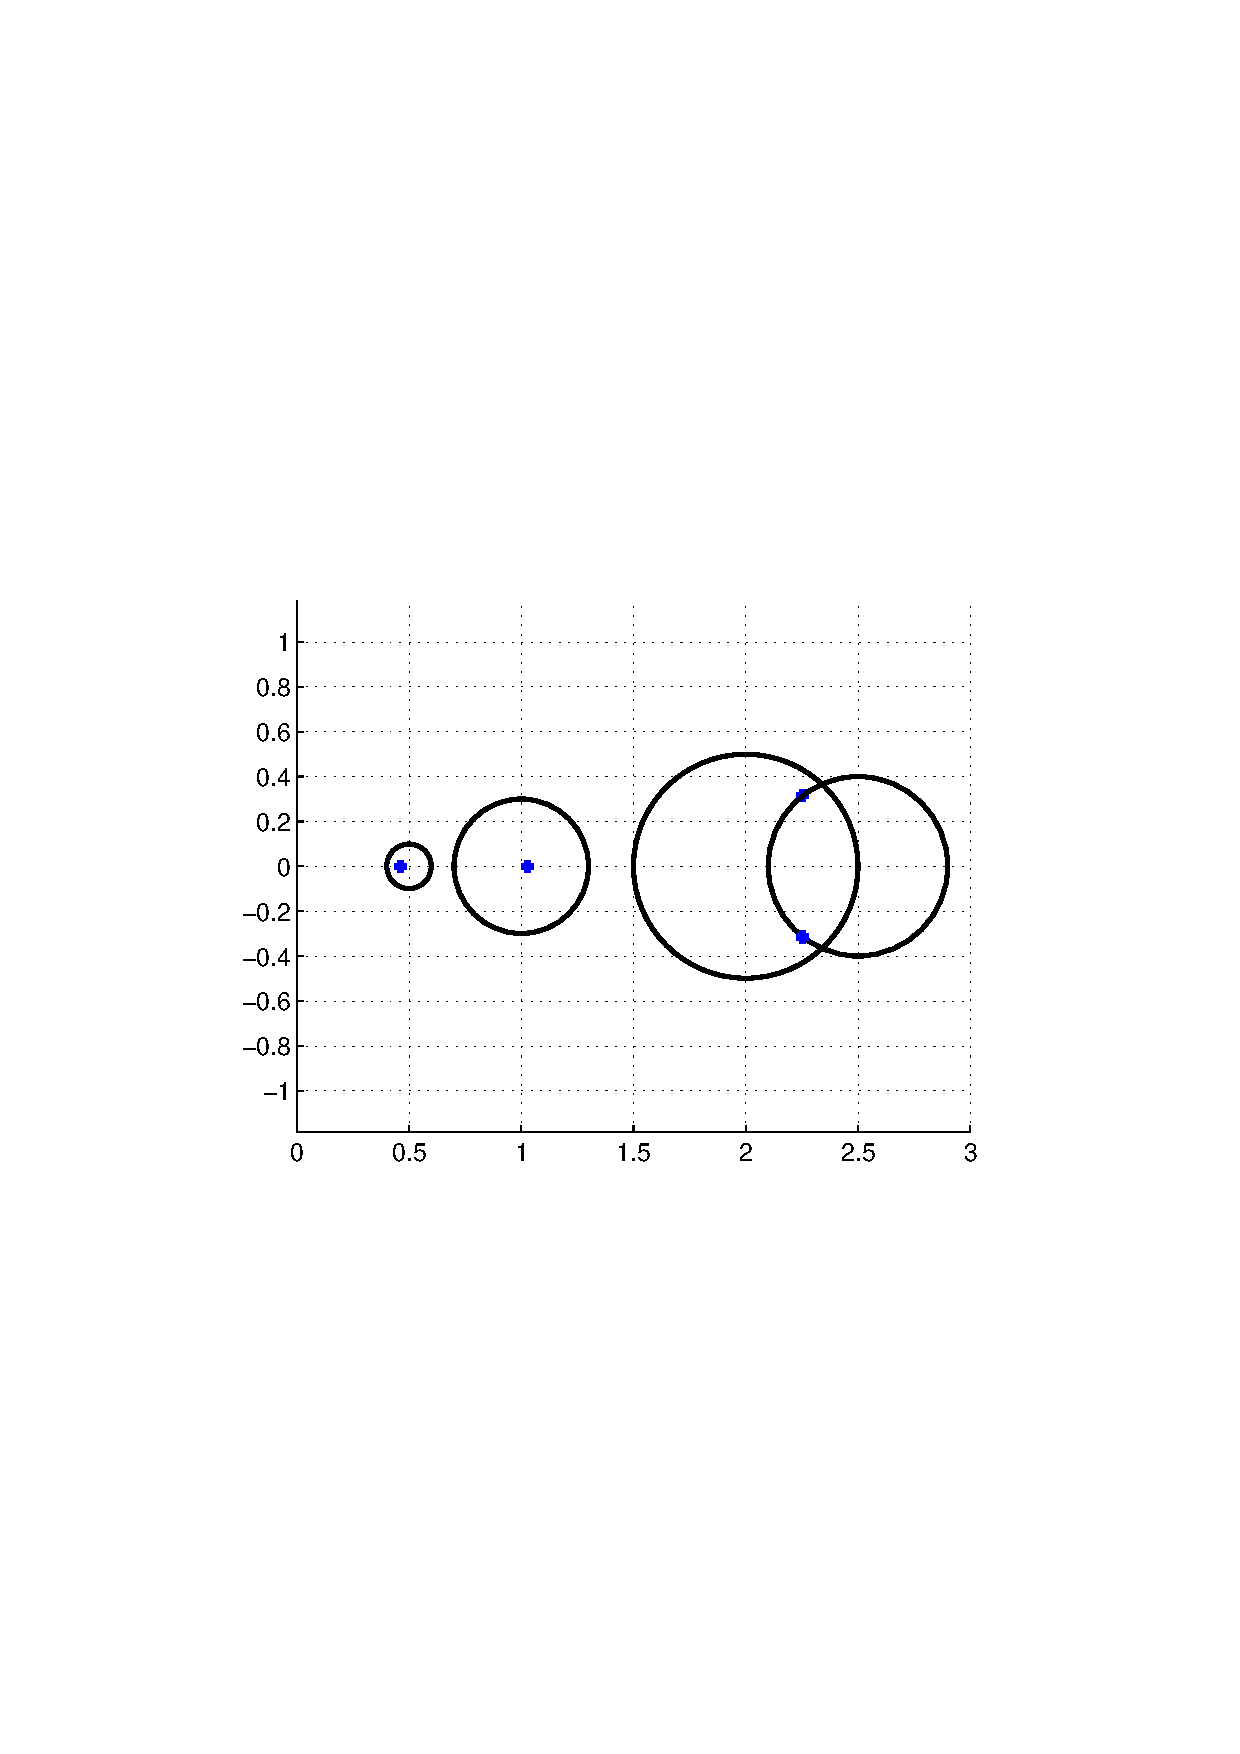
\includegraphics[width = \columnwidth]{gersh.pdf}
\end{minipage}

Sur cet exemple, les seuls disques qui contiennent deux valeurs propres sont
ceux qui s'intersectent. Les autres en contiennent une et une seule. Ce
phénomène, qui n'est pas anodin, est l'objet de l'exercice suivant.

\begin{exercice}
\label{ex:gersh} On note $\mathcal E$ une composante connexe de $\mathcal
G(A)$ et $p$ le nombre de disques $D_i$ inclus dans $\mathcal E$. Ainsi, dans
l'Exemple, $\mathcal G(A)$ a 3 composantes connexes
\[
D_1 \ (p = 1),\quad D_2 \ (p = 1), \quad D_3 \cup D_4 \ (p= 2)
\]
Le but de l'exercice est de montrer que $\mathcal E$ contient exactement $p$
valeurs propres de $A$ (comptées avec leur ordre de multiplicité algébrique). 

A cet effet, on note $D$ la diagonale de $A$ et, pour tout $0 \leq r \leq 1$
\[
A_r = rA + (1-r)D
\]
On note enfin $m(r)$ le nombre de valeurs propres de $A_r$ dans $\mathcal E$.
On cherche donc à montrer : $m(1) = p$.
\begin{enumerate}
\item Démontrez que $m(0) = p$.
	\solution{\\ $m(0)$ est le nombre de valeurs propres de la matrice
		diagonale~$A_0=D$
	dans~$\mathcal{E}$ qui est~$p$ par hypothèse.}
\item Démontrez que $\mathcal G(A_r) \subset \mathcal G(A)$.
	\solution{\\ Ce sont les mêmes disques mais avec des rayons plus petits.}
\item {Supposez qu'il existe} $\gamma$ une arc simple $\mathcal C^1$ par
	morceaux orienté positivement séparant $\mathcal E$ (à l'intérieur) de
	$\mathcal G(A) \setminus \mathcal E$ (à l'extérieur). Démontrez que
\[
	m(r) = \frac1{2\pi i}\int_{\gamma} \frac{\chi'_{r}(z)}{\chi_{r}(z)}dz
\]
où $\chi_{r}$ est le polynôme caractéristique de $A_r$.
\solution{\\
	On rappelle que le {\bf résidu} d'une fonction méromorphe exprimée en série
	de Laurent~$f(z)=\sum_{n=-L}^\infty a_n(z-z_0)^n$
	est~$\mathrm{Res}_{z_0}(f)=a_{-1}=\frac1{2\pi i}\oint_{\partial\Omega}
	f(z)\ud z$
	ou~$\Omega$ est un voisinage autour de~$z_0$.  En particulier, si~$f$ a un
	zéro d'ordre~$n$ en~$z_0$ alors~$\mathrm{Res}_{z_0}\parens{f'/f}=n$.
	Le~{\bf théorème des résidus} dit que si~$f:\C\to\C$ est holomorphe
	sur~$\Omega\setminus\{z_1,z_2,\ldots\}$ alors~$\oint_{\partial\Omega} f(z)\ud z=2\pi
	i\sum_k\mathrm{Res}_{z_k}(f)$.

	Pour répondre à la question sur~$m(r)$, on prend une courbe de
	Jordan~$\gamma$ qui sépare~$\mathcal{E}$ de son complémentaire
	en~$\mathcal{G}(A)$, puis on applique le théoreme des résidus.  Ceci compte
	(avec multiplicité) les racines de~$\chi_r$ entoures par cette courbe, et
	donc dans~$\mathcal{E}$.
}
\item Déduisez que que $m$ est continue et concluez.
	\solution{\\
		L'expression qui définit~$m(r)$ est une intégrale d'une fonction continue
		et bornée évaluée sur un domaine bornée, avec un paramètre~$r$, donc la
		continuité suit par le théorème de convergence dominée.

		Finalement, si~$m$ est continue à valeurs entiers, elle est constante, et
		on a donc~$m(0)=p=m(1)$.
	}
%\item \textbf{Application.} On suppose que les disques $D_i$ sont deux-à-deux disjoints. Montrer que $A$ est diagonalisable.
%{\item Proposer une configuration où un tel arc $\gamma$ n'existe pas. Comment peut-on conclure dans ce cas ?}
\end{enumerate}
\end{exercice}

Ce résultat donne des critères puissants:

\begin{corollary}
	Si les disques de Gershgorin d'une matrice sont deux-à-deux disjoints alors
	la matrice est diagonalisable.
\end{corollary}

\begin{proposition}
	Soit~$A$ une matrice irréductible et fortement diagonale dominante
	($\ \abs{a_{ii}}\ge\sum_{i\neq j}\abs{a_{ij}}$ avec au moins une inégalité
	stricte).  Alors~$A$ est inversible.  Si~$A$ est réductible en~$k$ blocs,
	une condition suffisante d'inversibilité est qu'il y ait~$k$ inégalités
	strictes, une dans chaque bloc.
\end{proposition}

%Citons pour finir un résultat de  \cite{serre2001} sur le domaine de
%Gershgorin d'une matrice $A$ \emph{irréductible} : si une valeur propre est
%sur la frontière de $\mathcal G(A)$, c'est un point d'intersection de tous
%les cercles.
Citons enfin le
% théorème de Gauss-Lucas
\begin{exercice}[Théorème de Gauss-Lucas]
	Les racines d'un polynôme dérivé~$P'$ sont dans l'enveloppe convexe des
	racines de~$P$.
\end{exercice}

\paragraph{Éléments singuliers}
Les éléments propres sont définis seulement pour les matrices carrées.
Encore, les théorèmes les plus intéressants sur les éléments propres portent
seulement sur les matrices hermitiennes.  On peut résoudre tout à coup ces
deux contraintes en considérant la matrice~$A^*A$ associée à toute matrice
rectangulaire~$A\in\M_{p,q}(\K)$.  Observons que~$A^*A$ est carrée et
hermitienne, et par le théorème spectral elle diagonalise avec des valeurs
propres réels~$\ge 0$.

\begin{definition}
	Les \emph{valeurs singulières} d'une matrice~$A\in\M_{p,q}(\K)$ sont les
	valeurs propres de la matrice~$A^*A$.  On les
	écrit~$\sigma_i(A)=\sqrt{\lambda_i(A^*A)}$ pour~$i=1,\ldots q$,
	typiquement par ordre décroissant~$\sigma_1\ge\cdots\ge\sigma_q\ge0$.
\end{definition}

\begin{proposition}
	\label{prp:singular}
	Les valeurs singulières d'une matrice sont toujours des nombres réels
	non-négatifs.  Le nombre de valeurs singulières différentes coïncide avec
	le rang de la matrice.  Pour une matrice hermitienne, les valeurs
	singulières sont ses valeurs propres en valeur absolue.
\end{proposition}

\begin{exercice}
	Démontrer la proposition~\ref{prp:singular}.
\end{exercice}

Plus tard, on verra que toute matrice~$A\in\M_{p,q}$ admet
une~\emph{décomposition en valeurs singulières} (SVD) de la forme~$A=U\Sigma V$,
où~$\Sigma\in\M_{p,q}(\R)$ est diagonale avec valeurs singulières de~$A$
sur sa diagonale, et les matrices~$U,V$ sont unitaires de taille~$p$ et~$q$
respectivement.


\subsection{Décomposition polaire}

Rappelons que~$\UU_n$ est le groupe des matrices unitaires ($A^*A=I$)
et~$\HH_n^{++}$ est l'ensemble des matrices hermitiennes ($A^*=A$) définies
positives~($\x^*A\x\ge 0$).  Pour~$n=1$ l'ensemble~$\UU_1$ sont les nombres
complexes de la forme~$e^{in\theta}$ et l'ensemble~$\HH_1^{++}$ sont les réels
positifs.  Tout élément~$z$ de~$\C\setminus\{0\}=\GL_1(\C)$ peut s'écrire de
forme unique comme~$z=re^{i\theta}$ avec~$r>0$.  Cette~\emph{décomposition
polaire} a un analogue direct avec les matrices.

\begin{theorem}[décomposition polaire]
	\label{thm:polaire}
	Toute matrice inversible~$A\in\GL_n(\C)$ admet une~\emph{décomposition
	polaire}
	unique~$A=HQ$ avec~$H\in\HH_n^{++}(\C)$ et~$Q\in\UU_n(\C)$.
	L'application~$A\mapsto(H,Q)$ est un homéomorphisme entre~$\GL_n(\C)$
	et~$\HH_n^{++}(\C)\times\UU_n(\C)$.\\
	Si~$A$ est réelle, alors~$H$ et~$Q$ le sont
	aussi (et donc~$H\in\SSS^{++}_n(\R)$ et~$Q\in\OO_n(\R)$).
\end{theorem}

\begin{exercice}
	Démontrez le théorème \ref{thm:polaire}.
\end{exercice}
\vspace{-1em}
Indications:
\begin{enumerate}
	\item Pour l'unicité, rappelez que le spectre d'une matrice
		unitaire sont des nombres complexes du cercle unité.
	\item Pour l'existence, diagonalisez la matrice hermitienne~$AA^*$ et
		utilisez le théorème spectral.
	\item Pour la continuité, observez que~$(H,Q)\mapsto HQ$ est une
		application continue (elle est un polynôme).  Il suffit de démontrer
		que l'inverse est séquentiellement continue, ce qui suit du fait
		que~$U_n$ est compact et de l'unicité de la décomposition.
	\item Pour le cas réel, la démonstration est parallèle au cas complexe.
\end{enumerate}
\solution{(sketch).  On démontrera en passant
l'existence et l'unicité de la racine carrée
de toute matrice~$H\in\HH_n^{++}$ (c'est à dire d'une
matrice~$h\in\HH_n^{++}$ telle que~$h^2=H$).

{\bf Existence.} La matrice~$AA^*$ est hermitienne définie positive.  Par le
théorème spectral, elle diagonalise avec un changement de base
unitaire:~$AA^*=U^*DU$ avec~$D$ diagonale strictement positive.  On définit
alors~$H=U^*\sqrt{D}U$, avec~$\sqrt{D}$ obtenue en faisant la racine carrée
terme à terme de~$D$.  Par construction~$H\in\HH_n^{++}$ et on vérifie
alors que~$H^2=HH^*=AA^*$.  Ensuite on définit~$Q=H^{-1}A$ et on a
alors~$Q^*Q=A^*H^{-2}A=A^*(AA^*)^{-1}A=1$, ce qui veut dire que~$Q\in\UU_n$.
{(\sl Note: la matrice~$H$ s'appelle une racine carrée de la
matrice~$AA^*$.)}

{\bf Unicité.} Soit~$A=H'Q'$ une autre décomposition polaire.  Alors la
matrice~$N=H^{-1}H'=Q(Q')^{-1}$ est unitaire, ce qui implique que le spectre
de~$N$ sont des unités complexes.  On montrera que le spectre est aussi réel
et positif, ce qui permettra de conclure que~$N$ est l'identité et que la
décomposition est unique.  Soit~$h$ une racine carrée (pas forcément unique à
ce moment) de la matrice~$H'$. On a donc que~$N$ est similaire à la
matrice~$N'=hH^{-1}S$.  Par sa définition, la matrice~$N'$ est hermitienne
définie positive, et par le théorème spéctral ses valeurs propres sont
réelles et positives, et il en est le même pour ceux de~$N$, ce qui permet de
conclure l'unicité de la décomposition polaire.
{(\sl Observation: la
	conclusion de cet argument prouve aussi que la racine carrée est unique
en~$\HH^{++}_n$, autrement on aurait plusieurs décompositions polaires!)}

{\bf Continuité.}  L'application~$(H,Q)\mapsto HQ$ est un polynôme de
degré~$2$ dans toutes ces composantes, donc elle est continue.  Pour
démontrer que l'inverse est continue, il suffit de démontrer qu'elle est
séquentiellement continue.  Soit donc~$A_n\to A$ une suite convergente de
matrices inversibles et~$H_nQ_n\to HQ$ la suite de décompositions polaires.
Soit~$R$ un point d'adhérence de la suite~$Q_n$ (qui existe parce que~$\UU_n$
est compact).  On ré-numérote les suites~$X_n$ par une suis-suite qui donne
la convergence vers~$R$.  On a donc que la suite~$H_n=A_nQ_n^*$ converge
vers~$S=AR^*$.  La matrice~$S$ est hermitienne et semi-définie positive~(parce
que~$\HH_n^+$ est fermé) et inversible (produit de deux matrices
inversibles), donc définie positive.  Alors~$SR=A$ est une décomposition
polaire de~$A$ et par unicité~$R=Q$ et~$S=H$.  La suite originale~$Q_n$
(avant re-numérotation) a au plus un point d'accumulation qui doit être~$Q$,
et donc elle converge vers~$Q$.  Enfin,~$H_n=A_nQ_n^*$ converge
vers~$AQ^*=H$ et on conclut.
}


La matrice~$H$ de la décomposition polaire s'appelle la~\emph{racine carrée}
de la matrice hermitienne~$AA^*$.  D'après cette démonstration, on a vu que
toute matrice hermitienne définie positive~$H$ admet une racine carrée~$h$
telle que~$h^2=H$.  On écrit parfois~$h=\sqrt H$.

La décomposition polaire représente toute transformation linéaire comme une
rotation~$Q$ suivie d'une application hermitienne~$H$ qui, par le théorème
spectral, est un~\emph{stretch} dans des directions orthogonales.  La
décomposition polaire n'est donc pas un résultat évident, que se passe-t-il
pour des matrices non-symétriques?

\begin{exercice}[difficile]
	Calculez la décomposition polaire de la
	matrice~$A=\parens{\begin{smallmatrix}1&1\\0&1\end{smallmatrix}}$.
\end{exercice}
\solution{$\ds
\begin{pmatrix}
1 & 1 \\
0 & 1
\end{pmatrix}
=
\begin{pmatrix}
{3}/{\sqrt{5}} & {1}/{\sqrt{5}} \\
1/{\sqrt5} & 2/\sqrt{5}
\end{pmatrix}
\begin{pmatrix}
2/\sqrt5 & 1/\sqrt5 \\
-1/\sqrt5 & 2/\sqrt5
\end{pmatrix}
$\\
(on peut trouver cette solution en diagonalisant d'abord la matrice
symétrique~$AA^*$ et suivant la preuve d'existence de la décomposition polaire)
}

\subsection{Décomposition en valeurs singulières}

\emph{\small Every matrix is diagonal, provided one uses the proper bases for
the domain and range spaces.\\ \hfill---Gilbert Strang}

Si~$A$ est une matrice inversible, elle a une décomposition
polaire~$A=HQ$ avec~$H$ hermitienne et~$Q$ unitaire.  Les valeurs propres
de~$H$ sont des réels positifs, dits les~\emph{valeurs singulières} de~$A$.
Par la preuve du théorème~\ref{thm:polaire}, les valeurs singulières sont les
racines carrées des valeurs propres de la matrice hermitienne~$A^*A$.

En fait, on peut définir les valeurs singulières d'une matrice~$A$
quelconque, pas forcément inversible, et même d'une matrice rectangulaire,
car~$A^*A$ et~$AA^*$ ont toujours les mêmes valeurs propres avec la même
multiplicité (sauf pour la multiplicité de $0$ si~$A$ est rectangulaire).

\begin{theorem}[décomposition en valeurs singulières, SVD]
	\label{thm:svd}
	Soit~$A\in\M_{p,q}(\C)$.  Alors il existent deux matrices unitaires~$U\in
	\UU_p(\C)$, $V\in\UU_q(\C)$ et une matrice quasi-diagonale~$\Sigma\in
	\M_{p,q}(\C)$
	\[
		\Sigma = \begin{pmatrix}
			\sigma_1 & & & & \\
			 & \ddots & & & \\
			 & & \sigma_r & & \\
			 & & & 0 & \\
			 & & & & \ddots
		\end{pmatrix}
	\]
	telles que~\fbox{$A=U\/\Sigma V^*$}.  Les nombres réels
	positifs~$\sigma_i$ sont les valeurs singulières non nuls de~$A$.  En
	particulier,~$r$ est le rang de~$A$. \\
	Si~$A$ est réelle alors on peut choisir~$U$ et~$V$ réelles orthogonales.
\end{theorem}

\begin{remark}
	Même pour les matrices carrées, la décomposition~$A=U\/\Sigma V$ ne dit pas
	que~$A$ soit diagonalisable sur une base de vecteurs orthogonaux: les
	rotations~$U$ et~$V$ sont a priori complètement différentes l'une de l'autre!
\end{remark}

\begin{remark}
	La décomposition SVD n'est pas du tout unique: même quand les
	les~$\sigma_i$ sont ordonnées et différentes, et la matrice est carrée, on
	peut multiplier les lignes et les colonnes de~$U$ et~$V$ par unités
	arbitraires.
\end{remark}

On trouvera la preuve complète de l'existence d'une décomposition SVD dans
tout livre moderne d'algèbre linéaire, par exemple [AK] ou [Serr].
Attention: les preuves paraissent souvent plus compliqués qu'elles ne le
sont.  Il est conseillé de commencer par le cas carré~$p=q$ inversible, puis
non inversible, puis le cas général.
%Ici on s'intéresse surtout aux applications de cette décomposition, qui est
%essentielle en calcul scientifique.

{\bf Schéma de la preuve du théorème~\ref{thm:svd}.}
Soit~$A$ une matrice~$p\times q$ de rang~$r$.
\begin{enumerate}
	\item La matrice~$A^*A$ est hermitienne et semi-définie positive, donc elle
		décompose comme
		\[
		A^*A=V\Lambda V^*
		=\sum_i\lambda_i\vv_i\vv_i^*
		=\sum_i(\sigma_i)^2\vv_i\vv_i^*
		\]
	Les colonnes orthogonales de~$\vv_i$ de~$V$ sont les vecteurs propres
	\item On a~$A^*A\vv_i=(\sigma_i)^2\vv_i$
	\item Si tous les~$\sigma_i$ sont positifs, posons
		$\uu_i=\tfrac1{\sigma_i}A\vv_i$.
	\item On vérifie que~$\uu_i$ est un vecteur propre unitaire de~$AA^*$.
	\item Soit~$\Sigma=\mathrm{diag}(\sigma_i)$.  On a alors
		\begin{align*}
			U & =A V\Sigma^{-1} \\
			U\/\Sigma & =A V \\
			A & =U\/A V^* \\
		\end{align*}
		ce qui conclut la preuve dans le cas non-singulier.
	\item Si les derniers~$\sigma_i=0$, on pet compléter la définition des
		colonnes de~$U$ en complétant une base orthonormée de~$\K^p$, puis on
		rajoute des lignes de~$0$ à~$\Sigma$.
\end{enumerate}

\bigskip

La SVD est la factorisation matricielle la plus importante, et la plus
utilisée en traitement du signal et en modélisation.  Notamment, pour
l'analyse en composantes principales et pour la définition la pseudo-inverse
(qui généralise le critère de moindres carrés).

{\bf SVD et décomposition polaire.}
%Le lien entre SVD et décomposition polaire
Soit~$A\in\GL_n(\C)$ et~$A=HQ$ sa décomposition polaire.  Par le théorème
spectral, la matrice~$H$ diagonalise dans une base orthogonale de vecteurs
propres~$H=PDP^*$ avec~$P\in\UU_n$ et~$D$ diagonale positive.  On a
donc~$A=PD(P^*Q)$, qui est une SVD.
Réciproquement, si~$A=U\/\Sigma V^*$ est une~SVD de~$A$,
alors~$A=(U\/\Sigma U^*)(UV^*)$ est la décomposition polaire de~$A$.  Ici on
voit que la décomposition polaire est possible pour matrices quelconque, pas
forcément inversibles ou même carrées.

{\bf SVD et éléments propres.}
Les valeurs singulières d'une matrice~$A$ sont les valeurs propres de~$A^*A$
ou de~$AA^*$.  Il est donc naturel qu'il y ait plein de relations entre
la SVD de~$A=U\/\Sigma V^*$ et ses éléments propres.  On les voit en re-écrivant
les matrices~$A^*A$ et~$AA^*$ à partir de la SVD:
\begin{align*}
	A^*A & = V\Sigma^*U^* U\Sigma V^* = V(\Sigma^*\Sigma)V^* \\
	AA^* & = U\Sigma V^* V\Sigma^* U^* = U(\Sigma\Sigma^*)U^*
\end{align*}

ainsi, les colonnes de~$V$ (vecteurs singuliers à droite) sont vecteurs
propres de~$A^*A$, et les colonnes de~$U$ (vecteurs singuliers à gauche) sont
vecteurs propres de~$AA^*$.
Quand~$A$ est hermitienne semi-définie positive, alors sa
diagonalisation~$A=UDU^*$ est une SVD.


\subsection{Pseudo-inverse de Moore-Penrose}

Si~$Ax=b$ est un système linéaire avec~$A$ carrée et inversible la solution
du système est donnée par~$x=A^{-1}b$.  La notion de pseudo-inverse (de
Moore-Penrose) permet de traiter le cas général, avec une matrice peut-être
rectangulaire, peut-être de rang incomplet.

\begin{definition}[pseudo-inverse]
	\label{def:pseudoinv}
	Soit~$A\in\M_{p,q}(\C)$ et~$A=U\/\Sigma V^*$ une SVD,
	avec~$U\in\UU(p)$, ~$V\in\UU(q)$
	et~$\Sigma=\parens{\begin{smallmatrix}D&0\\0&0\end{smallmatrix}}$.
	La~\emph{pseudo-inverse} de~$A$ est la matrice~$A\in\M_{q,p}(\C)$ définie
	par
	\[
		A^+=V\Sigma^+ U^*
		\qquad
		\textrm{avec}
		\qquad
		\Sigma^+=\begin{pmatrix}D^{-1}&0\\0&0\end{pmatrix}
	\]
\end{definition}

\begin{remark}
	Il se trouve que la pseudo-inverse ne dépend pas du choix de la SVD.
	C'est le théorème de Penrose, selon lequel on peu utiliser les
	propriétés ci-dessous comme la définition de~$A^+$.
\end{remark}

\begin{exercice}
	\label{ex:pseudoinv}
	Soit~$A\in\M_{p,q}(\C)$ et~$A^+\in\M_{q,p}(\C)$ sa pseudo-inverse.  Alors
	\begin{align*}
		& AA^+A=A \\
		& A^+AA^+=A^+ \\
		& (AA^+)*=AA^+ \\
		& (A^+A)*=A^+A
	\end{align*}
	De plus quand~$A$ est réelle alors~$A^+$ l'est aussi.
\end{exercice}
\solution{
	Ces quatre propriétés sont conséquence directe de la
	définition de la pseudo-inverse à partir de la SVD.  Par exemple la première
	propriété:
	\[
		AA^+A=(U\Sigma V^*)(V\Sigma^+ U^*)(U\Sigma V^*)=U\Sigma V^*=A
	\]
	du fait que~$\Sigma\Sigma^+$ est une semi-diagonale de~$1$.
}

La pseudo-inverse permet de donner une solution ``canonique'' au problème
général~$Ax=b$ par~$x=A^+b$.  Notons que cette solution est consistante avec
les constructions typiques:

\begin{exercice}$ $\\
	Si~$A\in\GL_n(\C)$ alors~$A^+=A^{-1}$.\\
	Si~$A\in\M_{p,q}(\R)$ de rang~$q\le p$ alors la solution de moindres carrés
	de~$\|Ax-b\|^2_2$ est donnée par~$x=A^+b$.
\end{exercice}
\solution{
	Si~$A\in\GL_n$ alors toutes les valeurs singulières sont strictement
	positive, et~$\Sigma^+=\Sigma^{-1}$ dans la définition de pseudo-inverse,
	et donc~$A^+=A^{-1}$.

	Si $A\in\M_{p,q}(\R)$ est de rang~$q\le p$ complet, alors la
	fonction~$x\mapsto\|Ax-b\|^2$ est une forme quadratique
	\[
		f(x)=x^\top A^\top Ax-2b^\top Ax-c
	\]
	dont la hessienne~$D^2f=2A^\top A\in\M_{q,q}(\R)$ est définie positive et le
	minimum est atteint au vecteur~$x$, solution unique de~$Df(x)=0$, c'est à
	dire le système linéaire~$A^\top Ax=A^\top b$.  On vérifie aisément
	que~$A^+=(A^\top A)^{-1}A$.
}

Le résultat suivant dit que la pseudo-inverse n'est pas une généralisation
arbitraire de~$A^{-1}$ (notamment, elle ne dépend pas du choix de la svd).

\begin{theorem}[Penrose 1955]
	Soit~$A^+$ une matrice qui satisfait les quatre propriétés de
	l'exercice~\ref{ex:pseudoinv}.  Alors~$A^+$ est la pseudo-inverse de~$A$
	selon la définition~\ref{def:pseudoinv}.
\end{theorem}

\begin{exercice}
	Calculez la pseudo-inverse des matrices suivantes
	\begin{itemize}
		\item La matrice zéro~$0\in\M_{p,q}(\K)$.
			\solution{$0^+=0^\top\in\M_{q,p}$}
		\item Un scalaire~$a\in\K=\M_{1,1}(\K)$.
			\solution{$a^+=\begin{cases}0 &\mathrm{si}\ a=0\\a^{-1}&\mathrm{si}\
				a\neq 0\end{cases}$}
		\item Un vecteur~$\x\in\K^n=\M_{n,1}(\K)$.
			\solution{$\x^+=\frac1{\Abs{\x}^2}\x^\top\in\M_{1,n}$ si~$\x\neq 0$}
		\item La matrice
			nilpotente~$A_1=\parens{\begin{smallmatrix}0&1\\0&0\end{smallmatrix}}$.
			\solution{$\parens{\begin{smallmatrix}0&1\\0&0\end{smallmatrix}}^+=
			\parens{\begin{smallmatrix}0&0\\1&0\end{smallmatrix}}$}
		\item La matrice
			singulière~$A_2=\parens{\begin{smallmatrix}1&1\\1&1\end{smallmatrix}}$.
			\solution{$\parens{\begin{smallmatrix}1&1\\1&1\end{smallmatrix}}^+=
			\frac14\parens{\begin{smallmatrix}1&1\\1&1\end{smallmatrix}}$}
		\item La matrice singulière~$\x\x^*\in\M_{n,n}(\K)$
			avec~$\x\in\K^n\setminus\{0\}$.
			\solution{\\
				$(\x\x^*)^+=\frac1{\Abs{\x}^4}\x\x^*$,
				cas particulier de~$(\x\y^*)^+=\frac{1}{\Abs{\x}^2\Abs{\y}^2}\y\x^*$
		}
	\end{itemize}
\end{exercice}


\clearpage
\subsection{Normes matricielles}

% def. norme matricielle

\begin{definition}[norme]
	Soit~$V$ un espace vectoriel sur~$\K$.
	Une~\emph{seminorme} sur~$V$ est une application~$p:V\to\R$
	qui satisfait les propriétés suivantes
	\begin{enumerate}
		\item[(i)] $p(\x+\y)\le p(\x)+p(\y)$
		\item[(ii)] $p\parens{\lambda\x}=\abs{\lambda}p(\x)$
	\end{enumerate}
	Si, de plus,~$p(\x)=0\implies\x=0$ on dit que~$p$ est une~\emph{norme}.
%	Soit~$V$ un espace vectoriel sur~$\K$.
%	Une~\emph{norme} sur~$V$ est une application~$p:V\to\R$
%	qui satisfait les propriétés suivantes
%	\begin{enumerate}
%		\item[(i)] $p(\x) = 0\ \implies\ \x=0$
%		\item[(ii)] $p(\x)\ge 0$
%		\item[(iii)] $p(\x+\y)\le p(\x)+p(\y)$
%		\item[(iv)] $p\parens{\lambda\x}=\abs{\lambda}p(\x)$
%	\end{enumerate}
%	Si toutes les propriétés sont satisfaites sauf (i) on dit que~$p$
%	est une~\emph{seminorme}.
\end{definition}

\begin{definition}[norme matricielle]
	Une~\emph{norme matricielle} sur les matrices carrées de dimension~$n$ est
	une application~$p:\M_n(\K)\to\R$ telle que
	\begin{enumerate}
		\item[(i)] $p$ est une norme sur l'espace vectoriel~$\M_n(\K)$
		\item[(ii)] $p(AB) \le p(A) p(B)$
	\end{enumerate}
\end{definition}

L'espace vectoriel~$\M_n(\K)$ est de dimension finie donc toutes les normes
sont équivalentes.  Ceci est très pratique : pour démontrer la convergence
d'une suite de matrices, il suffit de le faire avec la norme pour laquelle la
démonstration est plus facile.  Voyons quelques exemples de normes
matricielles.

% def. norme induite / norme d'opérateur , lemme de composition

\begin{definition}[norme induite]
	Soit~$\Abs\cdot$ une norme en~$\K^n$.  La~\emph{norme induite}
	par~$\Abs\cdot$ sur~$\M_n(\K)$ est la norme de l'opérateur
	linéaire %~$\K^n\to\K^n$
	associé à chaque matrice, notée~$\ABS\cdot$.  Ainsi
	\[
		\ABS{A}
		=
		\sup_{\x\neq0}\frac{\Abs{A\x}}{\Abs\x}
		=
		\max_{\Abs\x=1}\Abs{A\x}
	\]
	La norme induite par la norme~$\Abs\cdot_p$ de~$\K^n$
	s'écrit~$\ABS\cdot_p$.
\end{definition}

\begin{exercice}
	Démontrez que toute norme induite est une norme matricielle, et qu'elle
	satisfait les deux propriétés suivantes
	\begin{enumerate}
		\item[(i)] $\Abs{A\x}\le\ABS A\cdot\Abs\x$
		\item[(ii)] $\ABS I = 1$
	\end{enumerate}
\end{exercice}
%\solution{(1)
%}

\begin{exercice}
	Démontrez que la~\emph{norme de Frobenius} définie par
	\[
		\ABS A_F
		=
		\sqrt{\mathrm{tr}\parens{A^*A}}
		=
		\sqrt{\sum_{i,j}\Abs{a_{ij}}^2}
	\]
	est une norme matricielle mais n'est pas une norme induite.
\end{exercice}

% normes induites par la norme p=1,2,\infty

\begin{exercice}
	Vérifiez les caractérisations suivantes des normes induites classiques:
	\[
		\ABS A_1      = \max_j\sum_i\abs{a_{ij}}
		\qquad
		\ABS A_\infty = \max_i\sum_j\abs{a_{ij}} = \ABS{A^*}_1
		\qquad
		\ABS A_2      = \sqrt{\rho\parens{A^*A}} = \ABS{A^*}_2
	\]
\end{exercice}

% lien entre normes induites et rayon spectral

\begin{exercice}[Lien entre normes induites et rayon spectral]
	Démontrez que %les affirmations suivantes:
	\begin{enumerate}
		\item Pour toute matrice~$A\in\M_n(\K)$ on
			a~$\rho\parens{A^m}=\rho\parens{A}^m$ et~$\rho\parens{\lambda
			A}=\abs\lambda\rho\parens{A}$
		\item Si~$A$ est diagonale alors~$\ABS A_p=\rho(A)$
			pour~$1\le p\le\infty$.
		\item Si~$A$ est normale alors~$\ABS A_2=\rho(A)$.
		\item Si~$n>1$ alors le rayon spectral~$\rho$ n'est pas une norme
			sur~$\M_n(\K)$.
		\item Si~$\ABS\cdot$ est une norme induite sur~$\M_n(\C)$ alors
			\begin{equation}\label{eq:rholessthanABS}
				\rho(A)\le\ABS A
			\end{equation}
		\item${}^*$ L'équation~(\ref{eq:rholessthanABS}) est encore vraie pour
			une norme matricielle quelconque sur~$\M_n(\C)$, ou même
			sur~$\M_n(\R)$.
	\end{enumerate}
\end{exercice}

% théorème de Householder

L'inégalité~\ref{eq:rholessthanABS} dit que~$\rho(A)$ minore
l'ensemble~$\left\{\ABS A\ :\ \ABS\cdot\ \textrm{norme induite}\right\}$.  Le
théorème de Householder montre que c'est en fait la borne inférieure

\begin{theorem}[Householder]
	Pour toute matrice~$A\in\M_n(\C)$ et tout~$\epsilon>0$ il existe une norme
	induite~$\ABS\cdot_{A,\epsilon}$ telle que
	\begin{equation}\label{eq:rholessthanABS}
		\ABS A_{A,\epsilon}\le\rho(A)+\epsilon
	\end{equation}
\end{theorem}

\begin{exercice}[Démonstration du théorème de Householder]$ $
	\begin{enumerate}
		\item Soit~$\Abs\cdot_\alpha$ une norme en~$\K^n$ et~$P\in GL_n(\K)$.
			Démontrez que~$N(\x)=\Abs{P\x}_\alpha$ est une norme en~$\K^n$ et que
			sa norme induite est~$N(A)=\ABS{PAP^{-1}}_\alpha$.
		\item Soit~$A\in\M_n(\C)$ et~$\mu>0$, démontrez qu'il existe~$Q\in
			GL_n(\C)$ et~$D$ diagonale telles que~$Q^{-1}AQ=D+\mathrm{O}(\mu)$
		\item Démontrez le théorème de Householder.
	\end{enumerate}
\end{exercice}


% convergence de suites de matrices
%% \sum A^n  est convergente (vers 0) sii rho(A) < 1 et alors I-A est inversible
%% rho(A) = \lim |||A^n|||^(1/n)
%% exponentielle d'une matrice

\begin{exercice}[Convergence de suites de matrices]
	Démontrez les propositions suivantes:
	\begin{enumerate}
		\item Pour une norme induite, la condition~$\ABS A<1$ implique que~$I-A$
			est inversible, et l'inverse est la somme de la série
			normalement convergente~$\ds\sum_{k\ge0}A^k$.
		\item Pour toute matrice~$A\in\M_n(\K)$, la
			série~$\ds\sum_{k\ge0}\tfrac1{k!}A^k$ est normalement convergente.
			Sa limite~$e^A$ est une matrice inversible.
		\item $*$ Pour toute norme induite, on a
			toujours~$\ds\rho(A)=\lim_{k\to\infty}\ABS{A^k}^{\frac1k}$
	\end{enumerate}
\end{exercice}


\subsection{Conditionnement de matrices}

Beaucoup de problèmes de modélisation se réduisent à la solution de
l'équation~$Ax=b$.  L'opérateur~$A$ représente un système physique agissant
sur un état~$x$ que l'on veut connaître, et~$b$ est l'observation faite.
Dû à des erreurs de mesure, le vecteur~$b$ est souvent perturbé par le bruit,
ce qui donnera une valeur~$x$ inexacte.

{\bf Exemple.} (issu de [AK], section 5.3)
\[
A = \left(\begin{array}{cccc}
8 & 6 & 4 & 1 \\
1 & 4 & 5 & 1 \\
8 & 4 & 1 & 1 \\
1 & 4 & 3 & 6
\end{array}\right), \quad b =  \begin{pmatrix}8 \\ 10 \\ 2 \\ 6\end{pmatrix} \quad
\Rightarrow \quad
x = \begin{pmatrix}0 \\ 0 \\ 2 \\ 0\end{pmatrix}
\]
En modifiant légèrement~$b$, on obtient une solution très différente
\[
A = \left(\begin{array}{cccc}
8 & 6 & 4 & 1 \\
1 & 4 & 5 & 1 \\
8 & 4 & 1 & 1 \\
1 & 4 & 3 & 6
\end{array}\right), \quad b = \begin{pmatrix}8.05 \\ 10 \\ 2 \\ 6\end{pmatrix} \quad
\Rightarrow \quad x = \begin{pmatrix}2 \\ -5.225 \\ 5.5 \\ 1.4\end{pmatrix}
\]

Le~\emph{conditionnement} d'une matrice sert à étudier cet effet.

\begin{definition}[conditionnement d'une matrice]
	Soit~$A$ une matrice inversible et~$\ABS\cdot_\alpha$ une norme induite.  Le
	\emph{conditionnement} de~$A$ relatif à cette norme est
	\[
		\mathrm{cond}_\alpha(A) = \ABS A\ABS{A^{-1}}
	\]
\end{definition}

\begin{proposition}[conditionnement euclidien] Pour toute matrice
	inversible~$A$:
\[
\mathrm{cond}_2(A) = \sqrt{\frac{\lambda_{\max}(A^*A)}{\lambda_{\min}(A^*A)}}
\]
Si $A$ est normale
\[
\mathrm{cond}_2(A) = \frac{\abs{\lambda_{\max}(A)}}{\abs{\lambda_{\min}(A)}}
\]
Si $O \in U_n(\K)$ alors
\[
\mathrm{cond}_2(O) = 1, \quad \mathrm{cond}_2(AO) = \mathrm{cond}_2(OA) = \mathrm{cond}_2(A)
\]
\end{proposition}

%Les deux exercices suivants montrent que, lorsqu'on résout un problème de la
%forme~$Ax=b$, le conditionnement de~$A$ sert à majorer l'erreur de la
%solution à partir du bruit sur~$b$ ou même sur~$A$:
%\clearpage
Lorsqu'on résout un problème de la forme~$Ax=b$, le conditionnement de~$A$
sert à majorer l'erreur relatif de la solution~$x$.  On présente deux
versions de cette majoration, selon si on a des petites erreurs d'observation
(sur~$b$) ou de modélisation (sur~$A$):

\begin{exercice}[effet des erreurs d'observation]
	Soit~$\delta b$ une perturbation du second membre et~$\delta x$ l'erreur
	induit sur la solution, de sorte que~$A(x+\delta x)=b+\delta b$.  Démontrez
	que l'erreur relatif augmente d'un facteur au plus~$\mathrm{cond}(A)$:
	\[
		\frac{\Abs{\delta x}}{\Abs{x}}
		\le
		\mathrm{cond}(A)
		\frac{\Abs{\delta b}}{\Abs{b}}
	\]
	Démontrez que cette inégalité est optimale: il existe~$b$ et~$\delta
	b$ tels que l'égalité a lieu.
\end{exercice}


\begin{exercice}[effet des erreurs de modélisation]
	Soit~$\delta A$ une perturbation de la matrice et~$\delta x$ l'erreur
	induit sur la solution, de sorte que~$(A+\delta A)(x+\delta x)=b$.  Démontrez
	que l'erreur relatif augmente d'un facteur au plus~$\mathrm{cond}(A)$:
	\[
		\frac{\Abs{\delta x}}{\Abs{x+\delta x}}
		\le
		\mathrm{cond}(A)
		\frac{\ABS{\delta A}}{\ABS{A}}
	\]
	Démontrez que cette inégalité est optimale: il existe~$b$ et~$\delta
	A$ tels que l'égalité a lieu.
\end{exercice}

\begin{remark}
	D'après ces exercices, il est préférable que le conditionnement de $A$ soit
	proche de 1. Ceci est d'autant plus vrai pour les méthodes itératives où
	les erreurs sont propagées et amplifiées à chaque itération. La technique
	du \emph{préconditionnement} consiste à considérer un système linéaire
	équivalent
	\[
		PAx = Pb
	\]
	où la matrice~$P$, dite le~\emph{préconditionneur} a été choisie de façon
	que $\mathrm{cond} (PA) < \mathrm{cond}(A)$. Il existe plusieurs méthodes
	pour bien choisir $P$, par exemple si~$A$ est à diagonale dominante on peut
	choisir~$P=\mathrm{diag}(A)^{-1}$.
	On pourra consulter à ce sujet [AK, Chapitre 5].
\end{remark}

\begin{remark}
\label{rm:cond}
Les inégalités ci-dessus sont certes optimales, mais elles sont en général
très pessimistes (on dit aussi \emph{conservatives}). Ainsi dans
l'Exemple on a
\[
\frac{\Abs{\delta x}_{2}}{\Abs{x}{2}} \simeq 964 \frac{\Abs{\delta
b}_{2}}{\Abs{b}_{2}}
\]
ce qui fait déjà beaucoup, mais $\mathrm{cond}_2(A) \simeq 3199$.
\end{remark}

{\bf Exemple avec le laplacien 1D.}

On définit la matrice symétrique suivante, dite le <<laplacien discret 1D>>:
%(discrétisation par différences finies de la dérivée seconde):
\begin{equation}
\label{eq:A}
A = n^2 \left(\begin{array}{cccc}
2 & -1 & &  \\
-1 & \ddots & \ddots & \\
  & \ddots & \ddots & -1 \\
 & & -1 & 2
\end{array}\right) \in M_{n-1}(\R)
\end{equation}
Cette matrice apparait de manière naturelle quand on discrétise l'équation de
Laplace en dimension~$1$ (avec conditions de Dirichlet):
\begin{equation*}
	\begin{cases}
		u''(x)  = -f(x) & 0 < x < 1 \\
		u(x) = 0 & x\in\{0,1\}
\end{cases}
\end{equation*}
On fixe~$n\ge 1$ et on note
\[
	x_i = \frac{i}{n}, \quad 0 \leq i \leq n, \quad U = \begin{pmatrix}u(x_1)
		\\ \vdots \\ u(x_{n-1})\end{pmatrix} \in \R^{n-1}, \quad  b =
		\begin{pmatrix}f(x_1) \\ \vdots \\ f(x_{n-1})\end{pmatrix} \in \R^{n-1}
\]
Le problème discret est donc~$Ax=b$, avec une solution qui devrait
s'approcher de~$U$ (pour cela on va supposer que~$f$ est suffisamment
régulière).


\begin{exercice}[étude du Laplacien 1D]$ $
	\begin{enumerate}
		\item Démontrez que~$AU=b+\mathcal{O}\parens{\frac1{n^2}}$
		\item Démontrez que les valeurs propres de~$A$ sont $$\lambda_k = 4n^2
			\sin^2 \frac{\alpha_k}{2}, \quad \alpha_k =  \frac{k \pi}{n}, \quad
			1\leq k \leq n-1$$ avec pour vecteur propre associé $v_k = (\sin j
			\alpha_k)_{1 \leq j \leq n-1}$.\\
			Pouvait-on voir autrement que $A \in S_{n-1}^{++}(\R)$ ?
		\item Soit~$U_{\mathrm{approx}}$ la solution du système linéaire~$Ax=b$.
			Démontrez
			que $\Abs{U-U_{\mathrm{approx}}}_2=\mathcal{O}\parens{\frac1{n^2}}$
\item Démontrez que
\[
	\mathrm{cond}_2(A) \underset{n \rightarrow \infty}{\sim} \frac{4n^2}{\pi^2}
\]
de sorte que, quand $n$ est grand, la matrice est très mal conditionnée.
\item En notant $\x = U_{\mathrm{approx}}$, montrer que
\[
\lim_{n \rightarrow \infty } \frac{1}{n} \Abs{\x}^2 = \int_0^1 u^2(x)dx,
\quad \lim_{n \rightarrow \infty } \frac{1}{n} \Abs{b}^2 = \int_0^1 f^2(x)dx
\]
	\end{enumerate}
\item Montrer enfin qu'il existe une constante $c > 0$ indépendante de $n$ telle que
\[
\frac{\Abs{\delta\x}}{\Abs{\x}} \leq c \frac{\Abs{\delta b}}{\Abs{b}}
\]
de sorte que, même si la matrice est très mal conditionné, le problème est
très bien posé pour les conditions d'utilisation typiques.
\end{exercice}

%\begin{exercice}
%On va analyser la matrice $A$ du Laplacien discrétisé à la lumière de cette
%remarque.
%\begin{enumerate}
%\item Montrer que 
%\[
%	\mathrm{cond}_2(A) \underset{n \rightarrow \infty}{\sim} \frac{4n^2}{\pi^2}
%\]
%de sorte que, quand $n$ est grand, la matrice est très mal conditionnée.
%\item En notant $x = U_{\textrm{approx}}$, montrer que
%\[
%\lim_{n \rightarrow \infty } \frac{1}{n} \n{\xx}{2}^2 = \int_0^1 u^2(x)dx, \quad \lim_{n \rightarrow \infty } \frac{1}{n} \n{b}{2}^2 = \int_0^1 f^2(x)dx
%\]
%\item Montrer enfin qu'il existe une constante $c > 0$ indépendante de $n$ telle que
%\[
%\frac{\n{\delta x}{2}}{\n{\xx}{2}} \leq c \frac{\n{\delta b}{2}}{\n{b}{2}}
%\]
%\end{enumerate}
%\end{exercice}


% exemple de mauvais conditionnement

% exemple 2 (matrice de Hilbert)

% déf. nombre de condition (associé à une norme induite)

% prop. exemples de cond2 à partir des rayons spectraux

% perturbation de x selon la perturbation de b (lors de la solution de Ax=b)

% perturbation de x selon la perturbation de A (lors de la solution de Ax=b)

% observation que les inégalités sont ``pessimistes''

% exemple de la dérivée seconde discrète

\clearpage

\section{Méthodes directes}

Nous présentons trois méthodes directes de résolution de systèmes linéaires:
la factorisation LU (qui est la version matricielle de l'élimination
Gaussienne), la factorisation de Cholesky (valable seulement pour matrices
symétriques) et la factorisation QR (basée sur le procédé d'orthogonalisation
de Gram-Schmidt).  D'abord, on commence par un petit rappel de la complexité
des opérations matricielles basiques.

\subsection{Complexité}

% complexité = nombre de multiplications
La complexité d'un calcul est le nombre d'opérations élémentaires (additions,
soustractions,  produits et divisions) qu'il met en œuvre.  Une
simplification habituelle consiste à compter seulement le nombre de
multiplications.

{\bf Exemple.}
Un système linéaire triangulaire inversible
\[
\begin{array}{ccccc}
a_{1,1}x_1  & + \ldots +  & a_{1,n}x_n & = & b_1 \\
& \ddots & \vdots && \vdots \\
&& a_{n,n}x_n & =&  b_n
\end{array}
\]
est résolu avec l'algorithme suivant:
\begin{align*}
x_n & = \frac{1}{a_{n,n}}b_n \\
x_{n-i} & = \frac{1}{a_{n-i,n-i}}\left(
b_i - \sum_{j=n-i+1}^{n} a_{i,j}x_j
\right), \qquad 1 \leq i \leq n-1
\end{align*}
qui demande $\frac{n(n-1)}{2}$ additions, autant de multiplications et $n$
divisions. Sa complexité est donc ${n^2}/{2} + n/2$. En général, on considère
que $n$ est grand et on ne gardera que le terme dominant du développement
asymptotique.
\emph{On dit ainsi que la résolution d'un système triangulaire est en
$n^2/2$, ou encore en~$n^2$ (le terme constant est ignoré).}

\begin{exercice}Étudier la complexité des calculs suivants
	\begin{enumerate}
		\item La multiplication d'une matrice~$A\in M_n(\K)$ par un
			vecteur~$x\in\K^b$
		\item La multiplication (naïve) de deux matrices de~$M_n(\K)$
		\item Le produit scalaire de deux vecteurs de~$\K^n$
		\item La projection d'un vecteur de~$\K^n$ sur une droite
		\item Le déterminant d'une matrice par la formule de
			Leibniz~$|A|=\sum_\sigma(-1)^\sigma\prod_i a_{i,\sigma(i)}$
		\item Le déterminant, récursivement par la formule de
			Laplace~$\abs{A}=\sum_ia_{i,1}\abs{\mathrm{mineur}_{i,1}(A)}$
		\item La résolution d'un système linéaire par la règle de Cramer
		\item La résolution d'un système linéaire par élimination Gaussienne
		\item Calcul de l'inverse d'une matrice par élimination Gaussienne
		\item Le déterminant, après triangulation Gaussienne
	\end{enumerate}
\end{exercice}

Une construction classique~[Ser, 8.1.2] montre que les algorithmes
d'inversion d'une matrice peuvent être aussi rapides que ceux du produit de
matrices «\emph{Those who know how to multiply know also how to invert}».
Pourtant, la complexité du produit de matrices (i.e., le coût de l'algorithme
optimal) n'est pas connue, on a seulement de bornes supérieures.

Pour illustrer comment on pourrait faire moins que~$n^3$ opérations, montrons
la formule de Winograd pour calculer le produit de deux
matrices~$2\times 2$ avec~$7$ multiplications au lieu de~$8$:
\[
	\begin{pmatrix}
		a & b \\ c & d
	\end{pmatrix}
	\begin{pmatrix}
		A & C \\ B & D
	\end{pmatrix}
	=
	\begin{pmatrix}
		aA+bB & w+v+(a+b-c-d)D \\
		w+u+d(B+C-A-D) & w+u+v
	\end{pmatrix}
\]
avec~$u=(c-a)(C-D)$, $v=(c+d)(C-A)$ et~$w=aA+(c+d-a)(A+D-C)$.  Ce calcul
entraîne~$7$ multiplications et~$15$ additions.

\begin{exercice}
	Décrivez un algorithme avec~$O(n^{\log_2 7})\approx O(n^{2.8074})$ opérations
	pour multiplier deux matrices de taille~$n$.\\
	\emph{Indication: supposez que~$n=2^k$ et utilisez la
		multiplication par blocs récursivement pour arriver à une méthode
		avec~$7^k$ multiplications et~$5(7^k-4^k)$ additions.
	}
\end{exercice}

Les algorithmes de multiplication ``rapide'' de matrices sont un sujet de
recherche actuelle en informatique théorique.  Le record actuel est un
algorithme avec $n^{2.3728639}$ opérations [Le Gall, 2014].  En pratique, ces
algorithmes ne sont jamais utilisés parce que, même pour de matrices très
grandes, ils sont beaucoup plus lents que la méthode naïve.

Quelques commentaires au sujet de la complexité:

\begin{itemize}
	\item La tradition d'utiliser le nombre de multiplications pour évaluer la
		performance d'un algorithme n'a pas vraiment raison d'être: avec les
		processeurs d'aujourd'hui, les additions et multiplications en virgule
		flottante prennent essentiellement le même temps.
	\item Même le nombre total d'opérations n'est pas ce qui va déterminer la
		performance réelle d'un algorithme.  Pour les algorithmes implémentés en
		CPU, ce qui limite la performance n'est pas les calculs de la CPU, mais
		la communication entre la CPU et la mémoire vive.  Ainsi, les algorithmes
		les plus rapides sont ceux qui parcourent les données par ordre, en
		profitant toutes les couches de mémoire~\emph{cache} entre la RAM et la
		CPU.
	\item Pour les algorithmes en GPU, il est essentiel aussi d'avoir un
		algorithme~\emph{parallélisable}, qui fait exactement le même calcul en
		divisant les données d'entré en parties indépendantes.
	\item Du point de vue numérique on ne s'intéresse pas à la solution exacte
		théorique, mais à des solutions approchés avec une erreur~$\epsilon>0$.
		Ainsi, plutôt que le coût total de la méthode ce qui intéresse est
		le~\emph{taux d'approximation} des méthodes itératives: à quelle vitesse
		décroit l'erreur d'une méthode si on itère à partir d'une approximation
		grossière de la solution.
	\item Finalement, on travaille très rarement avec des matrices pleines très
		grandes.  Assez souvent (e.g., en EDP discrétisées), on a des
		matrices~\emph{creuses} ou tous les éléments de la matrice
		sont~$0$ sauf une quantité proportionnelle à~$n$ (au lieu de~$n^2$).
		Les structures de données et les algorithmes pour travailler avec
		matrices creuses sont toujours à la pointe de la recherche actuelle.
\end{itemize}

% complexité du produit naive de deux matrices quelconque = pqr
% complexité du produit naive de deux matrices carrées = n^3
% une multiplication en C vaut 4 multiplications en R
% résolution d'un système linéaire triangularire n^2/2 multiplications
% calcul naive d'un determinant n!
% calcul d'un determinant par élimination gaussienne n^2/2
% inversion d'une matrice par la règle de Cramér n!
% inversion d'une matrice par élimination Gaussienne n^3

% note: ``those who know how to multiply know how to invert''

% note: formule de Strassen

% note: recherche actuelle en multiplication de matrices (cf. produit Winograd)

% note: en réalité les multiplications sont plus rapides (!) que les additions

% note: en réalité ce qui importe aujourd'hui n'est pas autant le nombre
% total de calculs mais surtout la localité de l'accès à mémoire/possibilité
% de paraléliser

% note: matrices creuses



%\subsection{Exemples de problèmes linéaires}
%
%\subsection{Analyse matricielle}
%
%- groupes de matrices
%
%- théorème spéctral
%
%- rayon spéctral
%
%- normes matricielles
%
%- normes induites
%
%- théorème de Householder
%
%- conditionnement d'une matrice: définition, propriétés, exemple du laplacien
%à 5 points


\subsection{Méthode d'élimination de Gauss}

Le principe est de transformer~$Ax=b$ en un système
triangulaire équivalent. La méthode s'appuie sur le résultat suivant.

\begin{proposition}
Il existe $G \in\GL_n(\K)$ telle que $U = GA$ soit triangulaire supérieure.
\end{proposition}
Il ne reste alors plus qu'à résoudre le système triangulaire $Ux = Gb$

{\bf Algorithmique.}
On peut construire $G$ comme le produit d'au plus $n-1$ matrices triangulaires inférieures $T_1,\dots T_{n-1}$ et éventuellement de matrices de transposition s'il y a besoin de changer de \emph{pivot}. En pratique, le terme $Gb$ est mis à jour à chaque étape. On ne calcule pas explicitement $G$.

\begin{exercice}
Appliquez la méthode d'élimination de Gauss à
\[
A = \left(\begin{array}{ccc}
0 & 2 & 3 \\
1 & 4 & 1  \\
2 & 1 & -1
\end{array}\right), \quad b = \begin{pmatrix}1 \\ 8 \\5\end{pmatrix}
\]
Notez à chaque étape $k$ : le $k-$ième élément diagonal $q_k$, la matrice de
transposition $P_k$, le pivot $p_k$ (si $q_k \neq 0$, $P_k = I$ et $p_k =
q_k$), la matrice $T_k$.
\end{exercice}

{\bf Algorithmique.}
%On retiendra que
La méthode d'élimination de Gauss est en~$\displaystyle {n^3}/{3}$.

\begin{remark}
Les éléments diagonaux $u_{k,k}$ de $U$ sont les pivots $p_k$.
\end{remark}

\begin{remark}
Si $A$ est n'est pas inversible, la méthode d'élimination permet de rendre
$A$ triangulaire, mais $U$ n'est pas inversible. Aussi, $Ux = Gb$ n'a pas
nécessairement de solution.
\end{remark}

\begin{exercice}
Montrez que
\[
\det A = (-1)^p \prod_{k=1}^n u_{k,k}
\]
où $p$ est le nombre de matrices de transposition utilisées. La méthode
d'élimination de Gauss permet ainsi un calcul de déterminant en
$\displaystyle {n^3}/{3}$.
\end{exercice}

{\bf Algorithmique.}
Pour des raisons de stabilité numérique, il peut être utile de changer de
pivot lorsque $q_k$ est non nul mais petit. On peut prendre par exemple le
plus grand (en module) dans la sous-colonne $[k:n,k]$ (\emph{pivot partiel})
ou bien encore le plus grand dans la sous-matrice $[k:n,k:n]$ (\emph{pivot
total}). Un exemple concret est donné dans~[Cia,~p.78--79].

%\begin{remark}
%La méthode de Gauss permet aussi d'échelonner des systèmes linéaires
%non-carrés. On trouve une bonne présentation des systèmes échelonnés
%dans~\cite[Chapitre 4]{escofier2006}.
%\end{remark}

\subsection{Factorisation LU}

Si $q_k$ n'est jamais nul, il n'y a pas de matrice de transposition donc $G =
T_{n-1}\dots T_1 \in \TI$ et en notant $$L = G^{-1} = T_1^{-1} \dots
T_{n-1}^{-1} \in \TI$$ on a
\[
A = LU
\]
La \emph{décomposition} $LU$ de $A$ n'est donc rien d'autre que la mise en
\oe uvre de la méthode de Gauss dans ce cas. Comme on va le voir, le fait que
$q_k$ n'est jamais nul se lit sur les mineurs principaux de $A$.

\begin{theorem}
\label{th:lu}
On suppose que les mineurs principaux de $A$ sont tous non nuls. Il existe
alors un unique couple de matrices $(L,U)$ avec $L \in \TI^1_n(\K)$ et $U \in
\TS_n(\K)$ inversible telles que $A = LU$.
\end{theorem}
\begin{remark}
Les notations $L$ et $U$ se rapportent aux termes anglais \emph{lower} et
\emph{upper}.
\end{remark}
\begin{exercice}
On va prouver le Théorème~\ref{th:lu}. On reprend la méthode d'élimination de
Gauss.
\begin{enumerate}
\item (\emph{Unicité}). Sous réserve d'existence, montrez que la
	décomposition $LU$ est unique.
\item (\emph{Existence}) On suppose qu'il existe $k$ tel que
	$q_1,\dots,q_{k-1} \neq 0$ et $q_k = 0$. Montrez que le $k-$ième mineur
	principal de $A$ est nul. Conclure.
\item Réciproquement, on suppose que $A$ admet une telle décomposition.
	Montrez que les mineurs principaux de $A$ sont tous non-nuls.
\end{enumerate}
\end{exercice}

{\bf Algorithmique.} On pourrait croire que la factorisation $LU$ est plus
coûteuse que la méthode de Gauss puisqu'elle demande de calculer en outre la
matrice $L$. Il n'en est rien. La forme particulièrement simple des matrices
$T_i$ permet leur inversion par simple changement de signe de sa sous-colonne
non nulle. On obtient alors $L$ par concaténation de ces sous-colonnes (voir
[Cia.~p.83]).
%{Pour s'en convaincre, on pourra chercher à
%	calculer
%\[
%\left(\begin{array}{ccc}
%1 & 0 & 0 \\
%-2 & 1 & 0 \\
%-3 & 0 & 1
%\end{array}\right)^{-1} \quad \textrm{et} \quad \left(\begin{array}{ccc}
%1 & 0 & 0 \\
%2 & 1 & 0 \\
%3 & 0 & 1
%\end{array}\right)
%\left(\begin{array}{ccc}
%1 & 0 & 0 \\
%0 & 1 & 0 \\
%0 & 4 & 1
%\end{array}\right)
%\]
%}
Ainsi, la factorisation $LU$ est aussi en $n^3/3$.

On peut aussi calculer par récurrence les sous-matrices $[1:k,1:k]$ de $L$ et
$U$, cf.~[Serre,~chap.8]. Notons les $L_k,U_k$.
On cherche \emph{a priori} $L_{k+1},U_{k+1}$ sous la forme
\[
L_{k+1} = \left(\begin{array}{cc}
L_k & 0 \\
l^* & 1
\end{array}\right), \quad U_{k+1} = \left(\begin{array}{cc}
U_k & u \\
0 & z
\end{array}\right)
\]
avec $u,l \in \K^k$, $z \in \K$. On trouve $l$ et $u$ en résolvant deux
systèmes triangulaires de taille $k$, pour un coût en $k^2$. On a encore une
complexité en $n^3/3$.

\begin{remark}
Cette décomposition est utile lorsqu'on veut résoudre le système
\[
Ax = b
\]
pour plusieurs valeurs $b$. On résout alors deux systèmes triangulaires en cascade
\[
Ly = b, \quad Ux = y
\]
pour un coût en $n^2$. C'est le cas par exemple pour la résolution approchée
d'EDP %(Section~\ref{sec:edp})
ou bien du calcul de $A^{-1}$ présenté dans l'exercice qui suit.
\end{remark}

\begin{exercice}
On suppose que les mineurs principaux de $A$ sont tous non-nuls. Proposer une
méthode de calcul de $A^{-1}$ en $\displaystyle {4n^3}/{3}$. (\emph{En fait,
on peut réduire la complexité à $n^3$}).
\end{exercice}

%\begin{remark}
%\cite{serre2001} présente un algorithme astucieux de multiplication et d'inversion de matrice en $\mathcal O(n^{\log 7 / \log 2})$.
%\end{remark}

\subsection{Factorisation de Cholesky}

C'est une sorte de décomposition $LU$ pour les matrices hermitiennes définies
positives.

\begin{theorem}
\label{th:cholesky}
On suppose $A \in \HH^{++}_n(\C)$. Il existe une unique $B \in \TI^{++}_n(\C)$
telle que
\[
A = B B^*
\]
\end{theorem}

\begin{exercice}
On va prouver le Théorème~\ref{th:cholesky}.
\begin{enumerate}
\item Sous réserve d'existence, montrez l'unicité.
\item Justifiez que $A$ admet une décomposition $LU$ et que les $u_{k,k}$ sont strictement positifs.
\item On note 
\[
D = \left(\begin{array}{ccc}
\sqrt{u_{1,1}} & & \\
& \ddots & \\
& & \sqrt{u_{n,n}}
\end{array}\right)
\]
Montrez que $B = LD$ convient.
\end{enumerate}
\end{exercice}

{\bf Exemple.}
Établir la factorisation de Cholesky de la matrice
\[
A = \left(\begin{array}{ccc}
1 & 2 & 1 \\
2 & 13 & 2 \\
 1 & 2 & 2
\end{array}\right)
\]

{\bf Algorithmique.}
On retiendra que Cholesky est deux fois plus rapide que $LU$ (donc en
$n^3/6$) tout en offrant le même avantage de ramener à une cascade de deux
systèmes triangulaires
\[
By = b, \quad B^*x = y
\]
Aussi, on la préférera toujours à la décomposition $LU$ lorsque $A \in \HH^{++}_n(\C)$,
ce qui est le cas dans beaucoup d'applications
%(Cf. Section~\ref{sec:motiv linéaire}).

Notons que cette factorisation permet un calcul du déterminant dans
$\HH^{++}_n(\C)$ en $n^3/6$.

\begin{exercice}(moindres carrés et équation normale)
%On revient sur le problème aux moindres carrés (Section~\ref{sec:moindres
%carrés}).
On veut résoudre~$Ax=b$ avec~$A\in M_{p,q}(\K)$, $p\ge q$ et~$A$ de rang
complet~$q$ (problème sur-déterminé, en général sans solution).  Pour cela,
on cherche le~$x$ qui minimise l'erreur~$E(x)=\Abs{Ax-b}^2_2$.
\begin{enumerate}
	\item Vérifiez que~$E(x)$ est une fonction convexe et un polynôme de
		degré~$2$
	\item Démontrez que le minimum de~$E(x)$ est déterminé par l'équation
		normale~$A^*Ax=A^*b$.
	\item Donnez le coût de la résolution du problème à l'aide de la
		décomposition de Cholesky.
\end{enumerate}
%On suppose $n \ge m$ et $A$ de rang $m$. Donner le coût de la
%résolution du problème à l'aide de l'équation normale.
\end{exercice}

\begin{remark}
Il y a d'autres méthodes que l'équation normale pour résoudre un problème aux
moindres carrés. On pourra consulter à ce sujet~[AK,~chap.~7].
\end{remark}

La décomposition de Cholesky n'a pas une interprétation géométrique directe.
Son intérêt principal est qu'elle fournit des méthodes de solution de
systèmes linéaires très effectifs.  Même pour des systèmes non-symétriques,
on considère souvent leur équation normale pour pouvoir utiliser la
décomposition de Cholesky.  D'ailleurs, l'implémentation de la méthode est
des plus simples possibles (beaucoup plus simple que l'élimination Gausienne
avec des pivots).  Voici une implementation complète en langage~$C$:


\begin{Verbatim}[fontsize=\scriptsize]
        // compute a lower triangular matrix B such that B*B'=A
        void cholesky(int n, double B[n][n], double A[n][n])
        {
                // initialize matrix to 0
                for (int i = 0; i < n; i++)
                for (int j = 0; j < n; j++)
                        B[i][j] = 0;

                // standard Cholesky-Crout algorithm
                for (int i = 0; i < n; i++)
                for (int j = 0; j <= i; j++)
                {
                        double r = 0;
                        for (int k = 0; k < j; k++)
                                r += B[i][k] * B[j][k];
                        if (i == j)
                                B[i][j] = sqrt(A[i][j] - r);
                        else
                                B[i][j] = ( A[i][j] - r ) / B[j][j];
                }
        }
\end{Verbatim}

cette implémentation est simplement une copie des formules
\begin{align*}
	b_{ij} \ :=\  & \ds\frac{\ds a_{ij}-\sum_{k=1}^{j-1}b_{ik}b_{jk}}{b_{jj}} 
	\qquad j=1,\ldots, i-1
	\\
	& \\
	b_{ii} \ :=\  & \ds\sqrt{a_{ii}-\sum_{k=1}^{i-1}b^2_{ik}}
\end{align*}
qui remplissent la matrice~$B$ ligne par ligne.




\subsection{Factorisation QR}

\begin{theorem}
\label{thm:factorisation QR}
Soit $A \in\GL_n(\K)$. Il existe un unique couple de matrices $(Q,R)$ avec $Q
\in \UU(n)$ et $R \in \TS^{++}_n(\K)$ telles que
\[
A = QR
\]
Ceci définit un homéomorphisme de $\GL_n(\K)$ sur $\UU(n)\times\TS^{++}(\K)$.
\end{theorem}

\begin{exercice}
On va prouver le Théorème~\ref{thm:factorisation QR}.
\begin{enumerate}
\item Sous réserve d'existence, montrez l'unicité
\item Montrez l'existence. \emph{On pourra par exemple s'intéresser à la matrice $A^*A$}.
\item Montrez que la factorisation $QR$ définit bien un homéomorphisme.
\end{enumerate}
\end{exercice}

La méthode d'orthogonalisation de Gram-Schmidt, appliquée aux colonnes
de~$A$, fournit un algorithme pour calculer la décomposition~$A=QR$ (et
aussi, une preuve d'existence!).  Cependant, cette méthode est numériquement
très instable, et d'autres algorithmes sont utilisés en pratique pour obtenir
cette décomposition.  Les deux méthodes plus importantes sont
les~\emph{réflexions de Householder} et les~\emph{rotations de Givens}.

La décomposition~$QR$ est un outil essentiel pour la~\emph{méthode QR} pour
approcher itérativement tous les éléments propres d'une matrice.


%\begin{rem}
%C'est une version matricielle du procédé d'orthonormalisation de Gram-Schmidt appliqué aux colonnes de $A$.
%\end{rem}


\subsection{Exemples de factorisations}

Les factorisations suivantes sont très utilisées en~\emph{computer graphics}
et traitement d'images.  Vous pouvez démontrer leur existence et unicité
comme conséquences directes des factorisations antérieures.

\begin{proposition}[décomposition canonique d'une affinité]
	Toute application linéaire de déterminant positif~$A:\R^2\to\R^2$ qui n'est
	pas une similarité admet une décomposition unique
	\[
		A = H_\lambda R(\psi)T_tR(\phi)
		= \lambda
		\begin{pmatrix}\cos\psi & -\sin\psi\\\sin\psi & \cos\psi\end{pmatrix}
		\begin{pmatrix}t & 0 \\0 & 1\end{pmatrix}
		\begin{pmatrix}\cos\phi & -\sin\phi\\\sin\phi & \cos\phi\end{pmatrix}
	\]
	où~$\lambda>0$, ~$\lambda^2t$ est le déterminant de~$A$, les~$R$ sont
	matrices de rotation,~$\psi\in[0,\pi[$ et~$T_t$ est un~\emph{tilt}.
\end{proposition}
\solution{
	Par le théorème spectral, la matrice~$AA^\top$ diagonalise dans une base
	orthonormée:~$AA^\top=PDP^\top$ où~$P\in O_2$
et~$D=\left(\begin{smallmatrix}\lambda_1&0\\0&\lambda_2\end{smallmatrix}\right)$
avec~$\lambda_1\ge\lambda_2>0$.  On vérifie que la matrice~$Q=APD^{-1/2}$ est
orthogonale:
\[
	QQ^\top=APD^{-1/2}D^{-1/2}P^\top A^\top=APD^{-1}P^\top A^\top
	=A(A^\top A)^{-1}A^\top=I
\]
de sorte que~$A=QD^{1/2}P^\top$.  Pour conclure l'existence, il suffit de
démontrer que les matrices~$Q$ et~$P$ sont des rotations.  Commes les
déterminants de~$A$ et~$D$ sont positifs, les déterminants de~$Q$ et~$P$ ont
le même signe.  S'ils sont tous les deux~$-1$, on multiplie chacune de ces
matrices par la matrice
diagonale~$\left(\begin{smallmatrix}1&0\\0&-1\end{smallmatrix}\right)$ pour
obtenir des rotations.

%(
On peut aussi démontrer l'existence en itérant la décomposition~$QR$ et la
SVD:\\$A=QR=Q(UDV^\top)=(QU)DV^\top$.
%)

Pour démontrer l'unicité, supposons que~$
\lambda R_1\left(\begin{smallmatrix}t&0\\0&1\end{smallmatrix}\right)R_2=
\lambda' R_1'\left(\begin{smallmatrix}t'&0\\0&1\end{smallmatrix}\right)R_2'
$.  Puisque les valeurs propres sont uniques, il faut que~$\lambda=\lambda'$
et~$t=t'$.  On a ainsi~$R_1DR_2=R_1'DR_2'$, et, en arrangeant les facteurs, on obtient
deux relations équivalentes de la forme~$X_1D^2X_1^\top=D^2$
pour~$X_i=(R_i')^{-1}R_i$ matrices orthogonales.  Autrement,
dit~$X_1D^2=D^2X_1$, ou, plus explicitement
\[
	\begin{pmatrix}
		\alpha c & -\beta s \\
		\alpha s & \beta c \\
	\end{pmatrix}
	=
	\begin{pmatrix}
		\alpha c & -\alpha s \\
		\beta s & \beta c \\
	\end{pmatrix}
\]
En supposant que~$\alpha\neq\beta$, ceci implique que~$s=0$ (et~$c=1$), et
ainsi~$X_i=I$ et~$R_i=R_i'$.
}

La décomposition existe aussi si~$A$ est une similarité, mais dans ce
cas~$t=1$ et les angles ne sont pas uniques.
Cette décomposition modèle la transformation subie par un élément de surface
quand il est observé d'un point de vue oblique.

%\begin{center}
%	\includegraphics[width=0.2\linewidth]{affinedec.png}
%\end{center}


\bigskip

\begin{proposition}[rotation de Yaroslavski]
	Toute rotation admet une décomposition comme produit de trois~\emph{shears}
	\[
		\begin{pmatrix}\cos\theta & -\sin\theta\\\sin\theta & \cos\theta\end{pmatrix}
		=
		\begin{pmatrix}1&c\\0&1\end{pmatrix}
		\begin{pmatrix}1&0\\b&1\end{pmatrix}
		\begin{pmatrix}1&a\\0&1\end{pmatrix}
	\]
\end{proposition}

\begin{exercice}
	Exprimez~$a,b,c$ en fonction de l'angle~$\theta$.
\end{exercice}

Cette décomposition donne une méthode pour appliquer rotations sur les images
qui n'a pas de flou (contrairement à re-intérpoler l'image sur une grille
tournée).  L'idée est que le~\emph{shear} est essentiellement une opération
unidimensionnelle sur les lignes de l'image, et on peut appliquer des
translations très précises indépendamment sur chaque ligne.

\bigskip

Finalement, ce résultat classique en traitement de signal peut s'interpréter,
par exemple, en termes de la SVD:

\begin{proposition}
	Toute matrice circulante~\footnote{circulante = la colonne~$i$-ème est la
	permutation cyclique d'ordre~$i$ de la première colonne, de sorte que
toutes les diagonales sont constantes} diagonalise dans la base de la
transformée de Fourier discrète.
\end{proposition}

\clearpage
\section{Méthodes itératives}

Les méthodes itératives s'appuient sur la propriété du point fixe pour
les applications contractantes:

\begin{proposition}[point fixe de Banach]
	Soit~$F:V\to V$ une application~$k$-Lipschitzienne avec~$k<1$ sur un espace
	métrique complet~$V$.  Alors il existe un unique point~$x\in V$ tel
	que~$F(x)=x$.  De plus, pour tout~$a\in V$, la suite des itérées~$F^n(a)$
	converge vers~$x$.
\end{proposition}

Tout le jeu consiste, alors, à transformer chacun des problèmes~$Ax=b$
et~$Ax=\lambda x$ en problèmes de point fixe.  Parfois on peut appliquer
directement le théorème du point fixe de Banach, parfois des versions
légèrement différentes, comme celle de Browder (à ne pas confondre avec
Brouwer).


\begin{proposition}[point fixe de Bowder et Kirk]
	Soit~$C$ un sous-ensemble non-vide, borné, fermé et convexe d'un espace de
	Banach uniformément convexe, et~$F:C\to C$ une
	application~\emph{non-expansive}, c'est à dire,
	telle que~$\Abs{F^nx-F^ny}\le \Abs{x-y}$.  Alors~$F$ a un point fixe (pas
	forcément unique).  %De plus, toute suite d'iterés~$F^n(x)$ converge 
\end{proposition}

Le plus souvent, on donnera une construction particulière au cas de chaque
matrice, sans faire appel à ces résultats.


Nous présentons plusieurs types de méthodes itératives, par ordre croissant de
difficulté:
\begin{enumerate}
	\item Étant donnée une matrice carrée~$A\in M_n(\K)$, construire une
		suite~$(\lambda^k,\x^k)$ qui s'approche au valeur propre de magnitude
		plus grande et à son vecteur propre.
	\item Étant donné un système linéaire inversible~$A\x=b$, trouver une
		suite de vecteurs~$(x^k)$ qui s'approche à la solution du système.
	\item Étant donné une matrice diagonalisable~$A$, approcher l'ensemble
		entier de ses éléments propres.
\end{enumerate}


\subsection{Méthode de la puissance, puissance inverse}

Lest méthodes itératives les plus faciles à analyser sont les méthodes de
calcul des éléments propres extrémaux (avec le valeur propre le plus grand et
le plus petit).

L'idée de base est que la séquence d'applications itérées d'une
matrice~$A^nx$ s'approche rapidement vers une direction avec le valeur
propre la plus grande.

\subsubsection{Méthode de la puissance [AK]}
\paragraph*{Principe.} On construit une suite $(x^k)$ par récurrence
\[
x^0 \in \K^n, \quad x^{k+1} = \frac{Ax^k}{{\Abs{Ax^k}}}
\]

\begin{exercice}
\label{exo:puissance}
On suppose que $A$ est diagonalisable à valeurs propres réelles 
\[
|\lambda_1| \leq \dots \leq |\lambda_{n-1}| < {|\lambda_n|, \quad \textrm{avec} \quad \lambda_n > 0}
\]
On note $e_1,\dots,e_n$ une base de vecteurs propres \emph{normés} associés,
et on décompose $$x^0 = \sum_{i=1}^{n} \beta_i e_i$$
On suppose $\beta_n \neq 0$.
%{Quitte à changer $e_n$ en $\frac{\beta_n}{|\beta_n|}e_n$, on peut
%supposer $\beta_n > 0$.}
\begin{enumerate}
\item Montrer que
\[
	x^k = \mathrm{sgn}(\beta_n)e_n + \mathcal O(\tau ^k), \qquad \tau = \frac{|\lambda_{n-1}|}{|\lambda_n|}
\]
Ainsi, $x^k$ converge (au moins)  linéairement vers un vecteur propre de $A$
pour $\lambda_n${,} au taux de convergence $\tau$.
\item Montrer que
\[
\Abs{Ax^k}= \lambda_n + \mathcal{O} (\tau^k)
\]
\item On suppose $e_1,\dots e_n$ orthonormée. Montrer que
\[
\Abs{Ax^k} = \lambda_n + \mathcal{O} (\tau^{2k})
\]
\item L'hypothèse $\beta_n \neq 0$ est-elle vraiment restrictive ?
\item Adapter la méthode si $\lambda_n < 0$.
\end{enumerate}
\end{exercice}

\begin{remark}
En pratique, on arrête les itérations lorsque
\[
{\Abs{x^{k+1}-x^k}} \leq \epsilon
\]
où $\epsilon$ est un seuil fixé à l'avance.
\end{remark}

\subsubsection{Méthode de la puissance inverse [Serr]}

\paragraph*{Principe.}
On suppose $A$ inversible {avec $0 < |\lambda_1| < |\lambda_2|$} et on
applique la méthode de la puissance à $A^{-1}$. Ceci permet un calcul
approché de $\lambda_1$ et $e_1$ à un taux de convergence
$\frac{|\lambda_1|}{|\lambda_2|}$.

\begin{exercice}\label{exo:puissance inverse}$ $
\begin{enumerate}
\item On suppose qu'on connait une approximation $\mu$ d'une des valeurs propres $\lambda_i$ de $A$, avec 
\[
|\lambda_j - \mu | > |\lambda_i - \mu| > 0, \quad \forall j \neq i
\]
Montrer que la méthode de la puissance inverse appliquée à la matrice $A-\mu I$ permet un calcul approché de $\lambda_i$ avec un taux de convergence
\[
\frac{|\lambda_i - \mu|}{\min_{j \neq i}|\lambda_j - \mu|}
\]
C'est en fait le principal intérêt de la méthode de la puissance inverse.
\item \textbf{Application.} On suppose qu'un des disques de Gershgorin $D_i$
de $A$ n'intersecte aucun autre. Proposer une méthode de calcul approché de
l'unique valeur propre de $A$ contenue dans $D_i$.
\end{enumerate}
\end{exercice}

\subsection{Méthodes itératives de résolution: formulation générale}

%Ces méthodes ne permettent qu'un calcul approché de la solution $\xx$, mais
%sont rapides comparées aux méthodes directes.
Soit~$A\in\GL_n(\K)$ et~$b\in\K^n$, on veut trouver~$x\in\K^n$ tel
que~$Ax=b$.
Le principe de base est de décomposer $A$ en
\[
A = M - N
\]
avec $M$ inversible, de sorte que
\[
Ax = b \quad \Leftrightarrow \quad Mx = Nx + b \quad \Leftrightarrow \quad x = M^{-1}(Nx+b)
\]
La méthode itérative associée à la décomposition $A = M-N$ consiste alors à
choisir $x^0 \in \K^{n}$ et à calculer les itérés $x^k$ solution de
\[
Mx^{k+1} = (Nx^k + b)
\qquad\qquad
%\color{gray}
%x^{k+1} = M^{-1}(Nx^k + b)
\]
Ceci n'a d'intérêt que si $M$ facilite le travail (typiquement $M$ diagonale ou triangulaire). La pertinence de la décomposition se lit sur le rayon spectral de $M^{-1}N$.

\begin{proposition}
\label{prop:methodes_iteratives}
La suite $(x^k)$ converge vers la solution $x=A^{-1}b$ quelque soit $x^0$ si
et seulement si $\rho(M^{-1}N) < 1$. On dit alors que la méthode est
convergente.
\end{proposition}

\begin{exercice}
Prouver la Proposition \ref{prop:methodes_iteratives}. Montrer que la
convergence est au moins linéaire et donner le taux de convergence.
\end{exercice}


{\bf Algorithmique.}
En pratique on ne connait pas la solution $x$ (on en cherche une approximation !) donc on ne sait pas quel terme $x^k$ est satisfaisant. Un critère souvent utilisé est de s'arrêter lorsque
\[
\Abs{Ax^k-b} \leq \epsilon
\] 
où $\epsilon$ est un seuil défini à l'avance. On note $K$ le nombre d'itérations effectuées avant l'arrêt. En pratique, la complexité des méthodes itératives est en $Kn^2$. Elles sont donc intéressantes si $K \ll n$.

\begin{remark}
C'est une méthode de point fixe pour la fonction $x \mapsto (M^{-1}N x +b)$. L'inégalité $\rho(M^{-1}N) < 1$ équivaut au fait que la fonction est contractante.
\end{remark}


\subsection{Méthode de Jacobi}

Dans cette méthode $M$ est la diagonale de $A$, supposée inversible. Par exemple
\[
A = \left(\begin{array}{ccc}
1 & 2 & 0 \\
2 & 13 & 2 \\
 1 & 1 & 2
\end{array}\right)
, \quad M = \left(\begin{array}{ccc}
1 & 0 & 0 \\
0 & 13 & 0 \\
 0 & 0 & 2
\end{array}\right)
, \quad N = \left(\begin{array}{ccc}
0 & -2 & 0 \\
-2 & 0 & -2 \\
-1 & -1 & 0
\end{array}\right)
\]

\begin{exercice}
On suppose que $A$ est à diagonale strictement dominante. Montrer que la
méthode de Jacobi est convergente.
\end{exercice}

\subsection{Méthode de Gauss-Seidel}

Dans cette méthode $M$ est la partie triangulaire inférieure de $A$, par exemple
\[
A = \left(\begin{array}{ccc}
1 & 2 & 0 \\
2 & 13 & 2 \\
1 & 1 & 2
\end{array}\right)
, \quad M = \left(\begin{array}{ccc}
1 & 0 & 0 \\
2 & 13 & 0 \\
1 & 1 & 2
\end{array}\right)
, \quad N = \left(\begin{array}{ccc}
0 & -2 & 0 \\
0 & 0 & -2 \\
0 & 0 & 0
\end{array}\right)
\]

\begin{proposition}
\label{prop:gauss_seidel}
Si $A \in\HH^{++}_n(\K)  $ alors la méthode de Gauss-Seidel est convergente
\end{proposition}

\begin{exercice}
On va prouver la Proposition~\ref{prop:gauss_seidel}.
\begin{enumerate}
\item Montrer que $M^* + N$ est diagonale et définie positive.
\item On note $\Abs{x}_A = \sqrt{\pairing{Ax}{x}}$ la norme associée à $A$
	sur $\K^{n}$. Montrer que, pour tout $x \neq 0$
\[
\Abs{M^{-1}Nx}_{A}^2 < \Abs{x}_{A}^2
\]
\item Conclure
\end{enumerate}
\end{exercice}

\begin{remark}
On vient en fait de montrer que, de manière générale, la méthode est
convergente si $A \in \HH^{++}_n(\K)$ et $M^* + N \in \HH^{++}_n(\K)$.
\end{remark}
\begin{remark}
Un raffinement de la méthode de Gauss-Seidel consiste à pondérer la diagonale
de $A$ dans $M$ par un facteur $\frac{1}{\omega}$. Par exemple pour $\omega =
\frac{1}{3}$
\[
A = \left(\begin{array}{ccc}
1 & 2 & 0 \\
2 & 13 & 2 \\
1 & 1 & 2
\end{array}\right)
, \quad M = \left(\begin{array}{ccc}
3 & 0 & 0 \\
2 & 39 & 0 \\
1 & 1 & 6
\end{array}\right)
, \quad N = \left(\begin{array}{ccc}
2 & -2 & 0 \\
0 & 26 & -2 \\
0 & 0 & 4
\end{array}\right)
\]
C'est la \emph{méthode de relaxation} [Serr,~chap.~9]
convergente si et seulement si $|\omega-1| < 1$. L'idée est de choisir
judicieusement $\omega$ pour rendre $\rho(M^{-1}N)$ le plus petit possible,
accélérant ainsi la convergence.
\end{remark}

\subsection{Descente de gradient}

%\subsection{Descente de gradient à pas optimal}
Dans cette méthode $M = \frac{1}{\alpha} I$, où $\alpha \in \R^*$ est un
paramètre de réglage. Par exemple pour $\alpha = 0.1$
\begin{displaymath}
A = \left(\begin{array}{ccc}
1 & 2 & 0 \\
2 & 13 & 2 \\
 1 & 1 & 2
\end{array}\right)
, \quad M = \left(\begin{array}{ccc}
10 & 0 & 0 \\
0 & 10 & 0 \\
 0 & 0 & 10
\end{array}\right)
, \quad N = \left(\begin{array}{ccc}
9 & -2 & 0 \\
-2 & -3 & -2 \\
-1 & -1 & 8
\end{array}\right)
\end{displaymath}

\begin{exercice}
On suppose $A$ diagonalisable de valeurs propres $0 < \lambda_1 \leq \dots \leq \lambda_n$
\begin{enumerate}
\item Montrer que la suite des itérés est
\begin{displaymath}
x^{k+1} = x^{k} - \alpha (Ax^k -b)
\end{displaymath}
et justifier le nom de la méthode.
\item Montrer que la méthode du gradient converge si et seulement si $\displaystyle 0 < \alpha < \frac{2}{\rho(A)}$.
\item Montrer que la valeur
\begin{displaymath}
\alpha = \frac{2}{\lambda_1 + \lambda_n}
\end{displaymath}
minimise $\rho(M^{-1}N)$ qui vaut alors
\begin{displaymath}
\rho(M^{-1}N) = \frac{\lambda_n - \lambda_1}{\lambda_n + \lambda_1}
\end{displaymath}
\end{enumerate}
\end{exercice}

\begin{exercice}
On suppose $A \in \SSS^{++}_n(\R)$. Une variante de la méthode du gradient
consiste à faire varier $\alpha$ à chaque pas, en choisissant $\alpha_k$
qui minimise la fonction
\begin{displaymath}
\alpha \mapsto f(x_k - \alpha(Ax_k -b))
\end{displaymath}
où $f: x \mapsto \frac{1}{2}\pairing{Ax}{x} - \pairing{b}{x}$ est la fonction
convexe sous-jacente. Montrer que ce minimum est atteint en un unique point
\begin{displaymath}
	\alpha_k = \frac{\Abs{A x^k - b}^2}{\pairing{A(Ax^k-b)}{\,Ax^k-b}}
\end{displaymath}
C'est la méthode \emph{du gradient à pas optimal}.
\end{exercice}


\subsection{Gradient conjugué}
Les deux méthodes décrites ci-dessus de descente de gradient sont délaissées
au profit de l'algorithme beaucoup plus efficace du \emph{gradient conjugué}
[Hestenes-Steifel~1952], dans lequel les directions de descente sont
itérativement orthonormées pour le produit scalaire induit par $A$ sur
$\R^{n}$.
C'est en réalité une méthode directe qui atteint la solution exacte à
l'itération~$n$-ième.  Mais on l'utilise souvent comme méthode itérative dû à
ses bonnes propriétés d'approximation.
%Voir \cite[Chapitre 9]{allairekaber2002} pour un exposé détaillé. 

Soit~$A$ une matrice définie positive. %~$A\in\SSS^{++}_n(\R)$.
On veut résoudre le système linéaire~$Ax=b$.

{\bf Idée de la méthode.}
La fonction quadratique~$F:\R^n\to\R$
\begin{align*}
	F(z) &=\tfrac12(b-Az)^\top A^{-1}(b-Az)\\
	&=\tfrac12z^\top Az-b^\top z+\tfrac12b^\top A^{-1}b
\end{align*}
trouve son minimum sur la solution exacte~$z=A^{-1}b$.
Ceci suit du fait que~$A^{-1}$ est définie positive;
pour un vecteur~$z$ le~\emph{résidu}~$r=b-Az$ vaut zéro seulement pour~$z=x$.
En faisant une descente de gradient sur la fonction~$F$, on retrouve une
séquence  de vecteurs~$x_k$, résolvant itérativement des problèmes de
minimisation 1-dimensionnelle:
\[
	x_{k+1} : F(x_{k+1})=\min_u F(x_k+u r_kl)
	\qquad
	\mathrm{avec}\ r_k = DF(x_k)^\top=b-Ax_k
\]
Il se trouve que~$x_{k+1}$ peut se calculer explicitement et que la séquence
des~$r_k$ sont orthogonaux (pendant que~$r_k\neq0$).

{\bf Algorithme.}  Initialisation: soit~$x_0\in\R^n$ arbitraire
et~$p_0:=r_0:=b-Ax_0$.  Pour~$k=0,1,\ldots$:
\begin{enumerate}
	\item Si~$p_k=0$, on s'arrête: la solution est alors~$x_k$.
	\item calculer
		\begin{align*}
			\ds
			\alpha_k &:= \frac{r_k^\top r_k}{p_k^\top Ap_k} \\
			x_{k+1} &:= x_k+\alpha_kp_k \\
			r_{k+1} &:= r_k-\alpha_kAp_k \\
			\beta_k &:= \frac{r_{k+1}^\top r_{k+1}}{p_k^\top Ap_k} \\
		p_{k+1} &:= r_{k+1}+b_kp_k
		\end{align*}
\end{enumerate}

%\begin{remark}
%
%\end{remark}

\begin{exercice}[analyse du gradient conjugué]
	Soit~$A$ une matrice réelle définie positive et~$b\in\R^n$.   Alors pour
	toute initialisation~$x_0\in\R^n$ il existe un entier~$l\le n$ tel
	que~$p_l=0$, et les suites de vecteurs~$x_k,p_k,r_k$ satisfont les
	propriétés suivantes:
	\begin{enumerate}
		\item $Ax_l=b$
		\item $r_i^\top p_j=0$ pour~$0\le j\le i\le l$
		\item $r_i^\top p_i=r_i^\top r_i$ pour $i\le l$
		\item $p_i^\top A p_j=0$ pour $0\le i< j\le l$
		\item $p_i^\top A p_i>0$ pour $j\le l$
		\item $r_i^\top r_j=0$ pour~$0\le i< j\le l$
		\item $r_j^\top r_j>0$ pour~$j\le l$
		\item $r_i=b-Ax_i$ pour~$i\le l$
	\end{enumerate}
\end{exercice}

\begin{remark}
	On ne complète pas ici la preuve de convergence du Gradient Conjugué (qui
	est conséquence de ces propriétés).  Notons seulement que la convergence de
	cette méthode est quadratique (comme méthode d'approximation), et que les
	coefficients de la matrice~$A$ ne sont jamais utilisés directement.  Ceci
	rend le temps de calcul proportionnel à la~\emph{sparsité} de la
	matrice~$A$.
\end{remark}

%\subsection{Descente de gradient stochastique}

%\subsection{Méthode du gradient conjugué}



\subsection{Méthode QR}

La méthode~<<$QR$>> pour calculer~\emph{toutes} les valeurs propres consiste à
appliquer itérativement la décomposition~$QR$, et observer que la matrice
résultante s'approche à une diagonale avec les valeurs propres.

%\begin{theorem}
%\label{thm:factorisation QR}
%Soit $A \in GL_n(\kk)$. Il existe un unique couple de matrices $(Q,R)$ avec $Q \in \on$ et $R \in \tsp$ telles que
%\[
%A = QR
%\]
%Ceci définit un homéomorphisme de $GL_n(\kk)$ sur $\on \times \tsp$.
%\end{theorem}
%
%\exo On va prouver le Théorème~\ref{thm:factorisation QR}.
%\begin{enumerate}
%\item Sous réserve d'existence, montrer l'unicité
%\item Montrer l'existence. \emph{On pourra par exemple s'intéresser à la matrice $A^*A$}.
%\item Montrer que la factorisation $QR$ définit bien un homéomorphisme.
%\end{enumerate}
%
%\begin{rem}
%C'est une version matricielle du procédé d'orthonormalisation de Gram-Schmidt appliqué aux colonnes de $A$.
%\end{rem}
%

\paragraph*{Principe de la méthode.} On construit une suite de matrices $(A_k)$ par récurrence
\[
A_1 = A, \quad A_{k+1} = R_k Q_k
\]
où $(Q_k,R_k)$ est la factorisation $QR$ de $A_k$.

\begin{theorem}[Convergence de la méthode QR pour calculer les valeurs propres]
\label{thm:QR}
On suppose que $A$ est diagonalisable
\[
A = Y^{-1} D Y
\]
avec $D = \textrm{diag}(\lambda_1,\dots,\lambda_n)$
et
\[
|\lambda_1| > \dots > |\lambda_n| > 0
\]
On suppose en outre que $Y$ admet une décomposition $LU$. Alors, la partie triangulaire inférieure de $A_k$ converge vers $D$.
\end{theorem}

\begin{exercice}[long]
On va prouver le Théorème~\ref{thm:QR}. Pour simplifier on suppose les $\lambda_i$ réels strictement positifs. 
\begin{enumerate}
\item On note
\[
\Q_k = Q_1 \dots Q_k, \qquad \R_k = R_k \dots R_1
\]
Montrer que la factorisation $QR$ de la $k-$ième puissance de $A$ est 
\[
A^k = \Q_k \R_k
\]
\item On note $Y = LU$ la décomposition de $Y$. Pour simplifier on suppose que la diagonale de $U$ est strictement positive. On note encore
\[
Y^{-1} = QR
\]
la factorisation $QR$ de $Y^{-1}$. Montrer que 
\[
\Q_k \R_k = QR D^k L U
\]
\item Montrer que 
\[
D^k L D^{-k} = I +  \mathcal O \left(\sigma^k\right)
\]
où 
\[
\sigma = \max_j \frac{\lambda_{j+1}}{\lambda_j}
\]
En déduire
\[
\Q_k \R_k = QB_k R D^k U
\]
avec $B_k = I + o(1)$
\item On note $B_k = O_kT_k$ la factorisation $QR$ de $B_k$. Montrer que 
\[
\Q_k = Q O_k, \quad \R_k = T_k R D^k U
\]
\item Montrer enfin
\[
(Q_k) \rightarrow I, \quad (R_k) \rightarrow R D R^{-1}
\]
et conclure.
\end{enumerate}
\end{exercice}

\begin{remark}
Attention, dans l'exercice précédent la partie supérieure stricte de $A_k$ converge. Ce n'est pas le cas en général. Ceci est du au fait qu'on a supposé les valeurs propres de $A$ et les éléments diagonaux de $U$ strictement positifs. 
\end{remark}

{\bf Algorithmique.}
En pratique, le taux de convergence $\sigma$ peut être proche de 1, surtout
pour des matrices de grande taille. Pour accélérer la convergence, on peut
faire une approximation des valeurs propres par la méthode $QR$ puis utiliser
la puissance inverse comme présenté à l'Exercice~\ref{exo:puissance inverse}
pour les dernières itérations. Ceci permet en outre de calculer des vecteurs
propres.

{\bf Algorithmique.}
\begin{enumerate}
\item Le calcul de la factorisation $QR$ par le procédé de Gram-Schmidt est
	en $n^3$ mais cet algorithme a tendance à propager des erreurs d'arrondi.
	En pratique, on la calcule plutôt par l'algorithme de Householder
	[AK~chap.7], qui consiste à multiplier $A$ par $n-1$ matrices de symétrie
	orthogonale par rapport à des hyperplans bien choisis. Cette méthode est
	plus stable numériquement et plus rapide, en $2n^3/3$.
\item On pourrait penser à utiliser la factorisation $A = QR$ pour résoudre
	un système linéaire $Ax = b$. En effet, on est ramené au système
	triangulaire
\[
Rx = Q^* b
\]
Elle est rarement utilisée dans ce but car, même avec l'algorithme de
Householder, la factorisation $QR$ est deux fois plus lente que la méthode
d'élimination de Gauss.
\item
	Dans le cadre du calcul de valeur propres, où on itère des
	factorisation $QR$, il est préférable de mettre $A$ sous une forme réduite
	(dite \emph{de Hessenberg}) pour un coût en $5n^3/3$. Le calcul de la
	factorisation à chaque étape est alors en $4n^2$. On pourra consulter à ce
	sujet [Serr~chap.10].
\item On peut étendre la factorisation $QR$ à des matrices non-carrées. C'est
	une des méthodes de résolution d'un problème aux moindres carrés présentées
	dans [AK~chap.7].
\end{enumerate}

%\end{algo}
%
%\subsubsection{Autres méthodes}
%Citons enfin deux méthodes qui s'appliquent à des matrices symétriques réelles~\cite[Chapitre 6]{ciarlet1994}.
%\begin{itemize}
%\item Jacobi, qui permet de calculer les valeurs propres et vecteurs propres
%\item Givens-Householder,  qui s'appuie sur les suites de Sturm.
%\end{itemize}
%
%\bibliographystyle{alpha}
%\bibliography{../bibmath}
%
%\subsection{Méthodes de calcul de la SVD}
%
%- bidiagonalisation + méthode itérative, méthode QR
%
%%\subsection{Méthode QR}

\section{Exemples de modélisation}

\subsection{Stabilité d'une équation différentielle}
On considère une équation différentielle linéaire à coefficients constants
\begin{align*}
X'(t) & = AX(t), \quad t \in \R \\
X(0) & = X_0
\end{align*}
avec $A \in M_n(\K)$. Le spectre de $A$ renseigne sur la nature des solutions.
\begin{itemize}
\item si les valeurs propres de $A$ sont à partie réelle $<0$, $X(t)$ converge vers 0 (quand $t\rightarrow +\infty$) quel que soit $X_0$ . L'équation est dite \emph{asymptotiquement stable}.
\item si $A$ admet une valeur propre à partie réelle $> 0$, $|X(t)|$ diverge vers l'infini pour presque toutes les conditions initiales $X_0$. L'équation est dite \emph{instable}.
\end{itemize}

\begin{remark}
Si l'une des valeurs propres est à partie réelle nulle, il faut étudier
l'espace propre associé pour en savoir plus.
\end{remark}

\begin{center}
	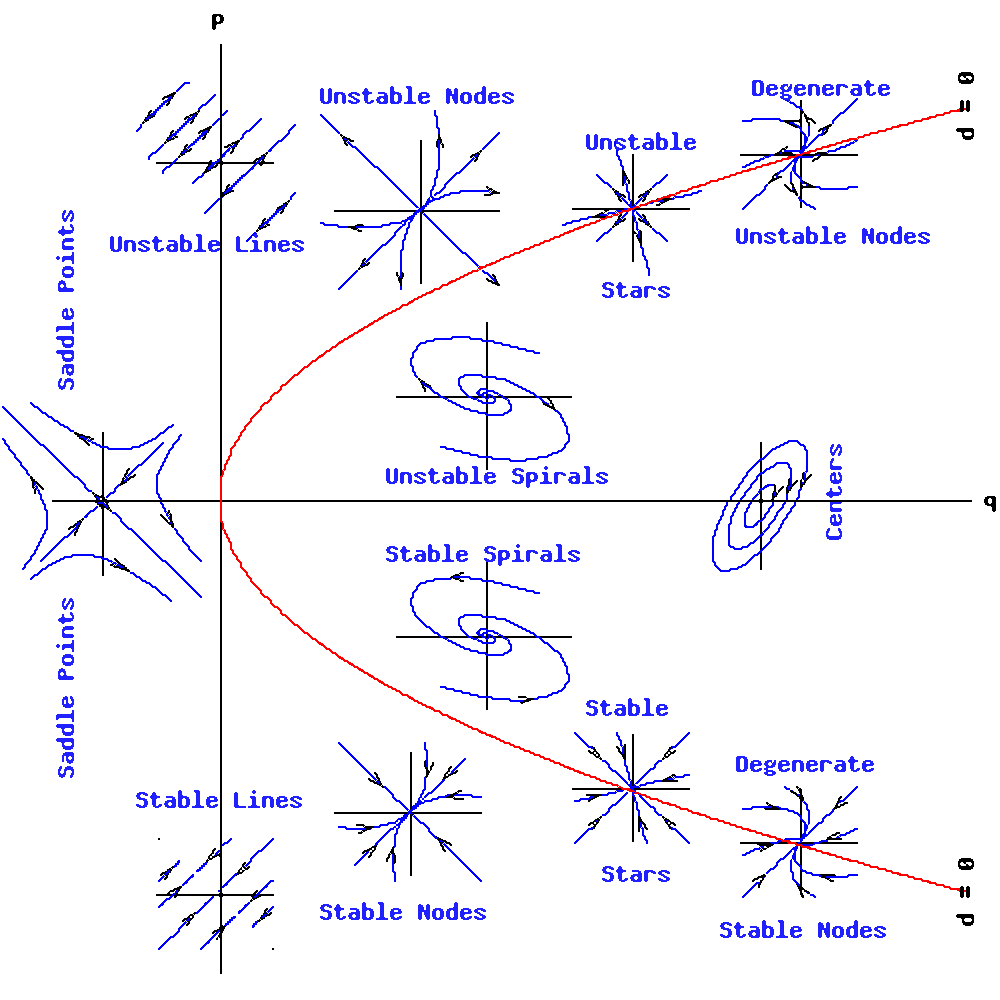
\includegraphics[width=0.57\linewidth]{flows2d.png}\\
	\scriptsize Diagramme de Poincaré (source:wikipedia)
\end{center}

%\subsection{Analyse en composantes principales}
%On considère un nuage de $m$ points de $\R^{n}$ 
%\begin{displaymath}
%X^k = (x^k_i)_{1 \leq i \leq n}, \quad 1 \leq k \leq m
%\end{displaymath}
%Il n'est pas aisé de manipuler des données que l'on ne sait pas visualiser.
%Aussi, on cherche à représenter ce nuage de points dans un espace de petite
%dimension $d$ (typiquement $d=2$ ou 3) en perdant ``peu'' d'information.
%Quitte à centrer les $X^k$, on considère que
%$$\displaystyle\sum_{k=1}^m X^k = 0$$
%On note $\Gamma \in M_n(\R)$ la matrice de covariance des $X^k$ définie par
%\begin{displaymath}
%\Gamma_{i,j} = \frac{1}{m} \sum_{k=1}^{m} x^k_i x^k_j
%\end{displaymath}
%La matrice ${\Gamma}$ est symétrique, positive. Notons $\lambda_1 \geq \dots \geq
%\lambda_n \geq 0$ ses valeurs propres et $V_1,\dots V_n$ une base orthonormée
%de vecteurs propres associés. Les $V_i$ représentent les axes principaux de
%$\Gamma$ (on dit aussi les \emph{composantes principales}). Le scalaire
%$\lambda_i$ est
%la variance (ou dispersion) du nuage de points dans la direction $V_i$. 
%
%Si $\lambda_i$ est petit, les points sont peu dispersés dans la direction
%$V_i$ et on ne perd pas grand chose à considérer que le nuage est contenu
%dans le plan orthogonal à $V_i$. On sélectionne alors les $d$ plus grandes
%valeurs propres $\lambda_1 \geq \dots \geq \lambda_d$ et on projette le nuage
%de points dans l'espace engendré par $V_1,\dots, V_d$ :
%\begin{displaymath}
%Y^k = \sum_{i=1}^{d} \pairing{V_i}{X^k} V_i
%\end{displaymath}
%On a ainsi ``compressé'' les $X^k$ en un nuage de points $Y^k$ en dimension $d$. Le taux de compression est défini par
%\begin{displaymath}
%\tau = \frac{\sum_{i=1}^{d} \lambda_i}{\sum_{i=1}^{n} \lambda_i}
%\end{displaymath}


%\subsubsection{Moteur de recherche}
%Un bon moteur de recherche se doit de classer les pages de la toile selon un ordre d'importance qui a du sens pour l'utilisateur. Une célèbre entreprise de la Silicon Valley créée en 1998 doit son succès à la pertinence de son algorithme PageRank, qui fonctionne selon le principe suivant. 
%
%Numérotons les pages de la toile de 1 à $n$. On note $x_i$ le score de la page $i$, $\mathcal E_i$ l'ensemble des pages pointées par $i$, $n_i = |\mathcal E_i|$ le nombre de ces pages. Le score est défini implicitement par
%
%\begin{equation}
%\label{eq:pagerank}
%x_i = \sum_{i \in \mathcal E_j} \frac{x_j}{n_j}
%\end{equation}
%Autrement dit, le score de la page $i$ est la somme des scores pondérés des pages pointant vers $i$. 
%
%Cette définition présente l'avantage du bon sens mais ne permet pas un calcul direct des $x_i$ puisqu'elle est implicite. On introduit alors la \emph{matrice d'adjacence} du web $A \in M_n(\rr)$ définie par
%\begin{align*}
%a_{i,j} & = \frac{1}{n_j} \quad \textrm{si $j$ pointe vers $i$} \\
%a_{i,j} & = 0 \quad \textrm{sinon}
%\end{align*}
%\begin{ex}
%\end{ex}
%\begin{center}
%\begin{tikzpicture}
%\node at (-70mm,0) {$
%A = \left(\begin{array}{ccc}
%0 & 0 & 1\\
%\frac{1}{2} & 0 & 0\\
%\frac{1}{2} & 1 & 0
%\end{array}\right)$};
%\node at (0,0) {\includegraphics[width = 0.4\columnwidth]{../figures/web}};
%\end{tikzpicture}
%\end{center}
%
%En notant $x = (x_i)_{1 \leq i \leq n} \in \r{n}$ \eqref{eq:pagerank} se réécrit au moyen de $A$ 
%\begin{displaymath}
%Ax = x
%\end{displaymath}
%Ainsi, trouver le score $x$ des pages de la toile revient à trouver un vecteur propre de $A$ associé à la valeur propre $1$. 
%
%\begin{rem}
%La matrice 
%\end{rem}

%\subsection{Vibrations d'un système mécanique [AK]}
%\begin{center}
%\begin{tikzpicture}
%\node at(0,0) {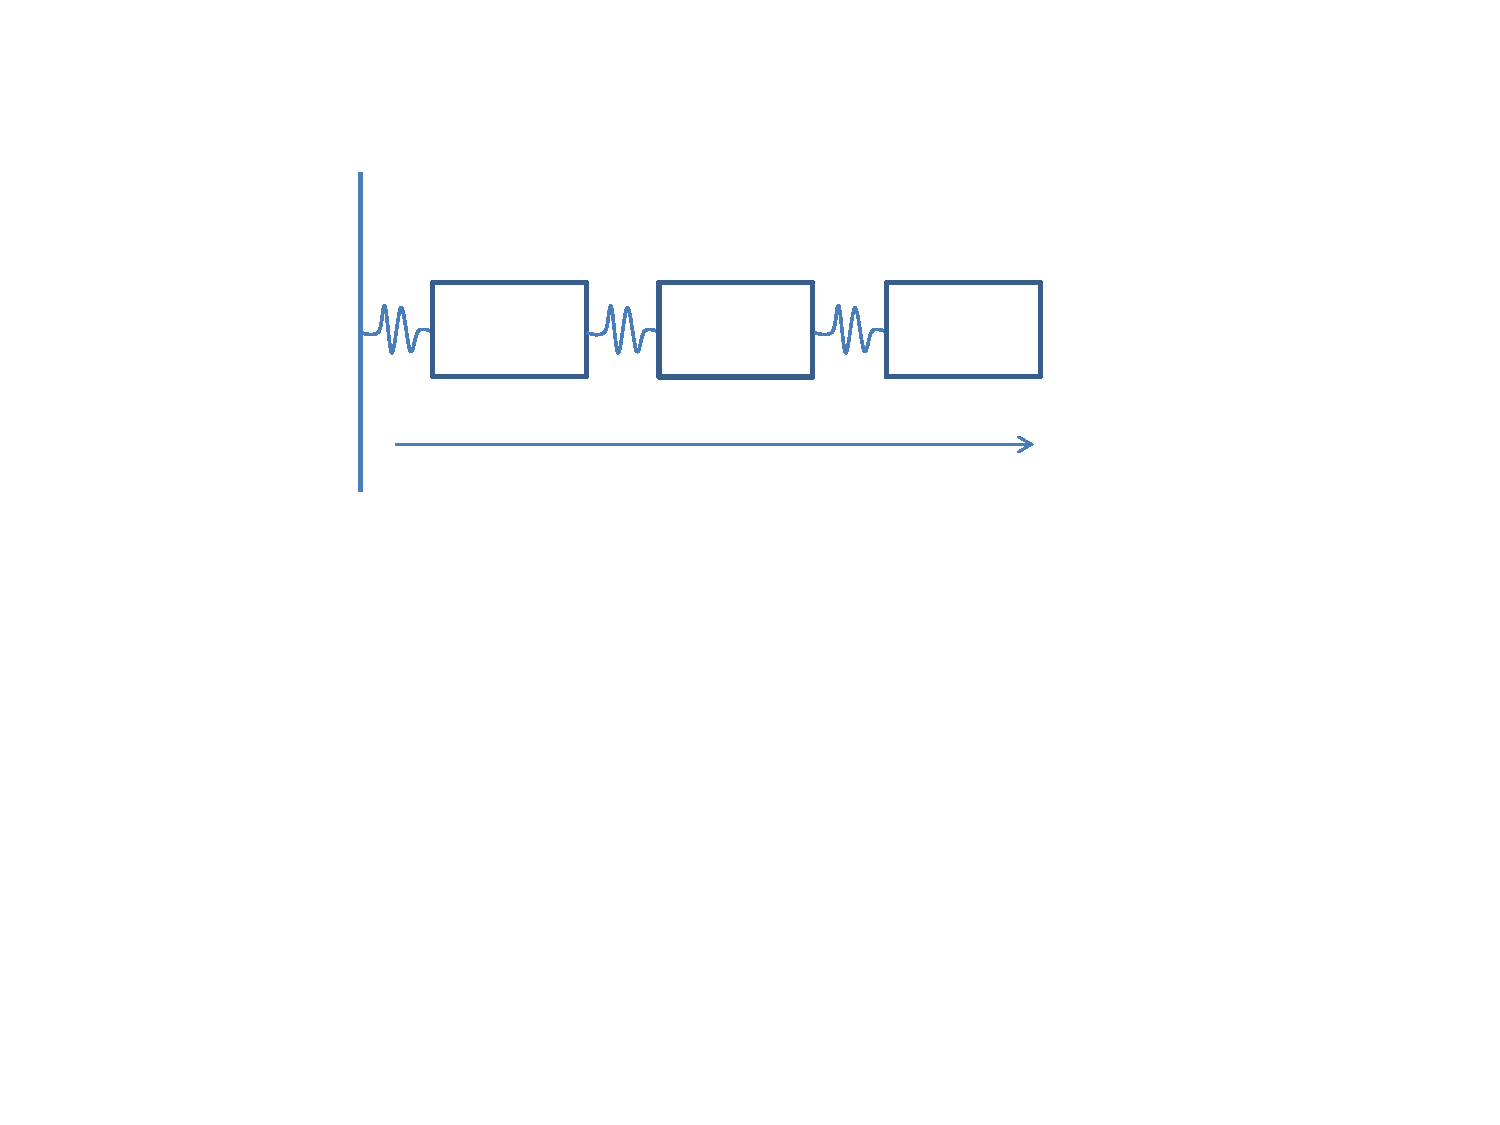
\includegraphics{masses_ressorts}};
%\node at(-51mm,8mm) {$k_1$};
%\node at(-13mm,8mm) {$k_2$};
%\node at(25.7mm,8mm) {$k_3$};
%\node at(6.5mm,-0.5mm) {$m$};
%\node at(-32mm,-0.5mm) {$m$};
%\node at(45mm,-0.5mm) {$m$};
%\node at(60mm,-20mm) {$x$};
%\end{tikzpicture}
%\end{center}
%Considérons un système unidimensionnel de trois masses $m$ reliées entre elles et à un support par des ressorts de constante de raideur $k_1,k_2,k_3$. On note $x_1, x_2,x_3$ le déplacement respectif des masses par rapport à leur position d'équilibre, $X = (x_1,x_2,x_3)$ satisfait l'équation différentielle
%\begin{displaymath}
%m \ddot X + K X = 0, \quad \textrm{avec} \ K = \left(\begin{array}{ccc}
%k_1 + k_2 & -k_2 & 0 \\
%-k_2 & k_2 + k_3 & -k_3 \\
%0 & -k_3 & k_3
%\end{array}\right)
%\end{displaymath}
%On cherche les pulsations propres du système c'est-à-dire les $\omega > 0$ telles qu'il existe une solution $X(t) = e^{i\omega t}X_0$. On a alors
%\begin{displaymath}
%K X_0 = m \omega^2 X_0
%\end{displaymath}
%Ainsi, la recherche des pulsations propres est équivalente à la recherche des valeurs propres de $K$. Cette méthode est utilisée pour calculer les pulsations propres d'un immeuble représenté par $n$ masses (plafonds) et ressorts (murs), en particulier pour prévoir son comportement en cas de séisme.

\subsection{Laplaciens discrets}


\begin{exercice}
On considère les trois matrices suivantes:
\[
	D_3=\left(\begin{smallmatrix}
		-2 & 1 & 0 \\
		1 & -2 & 1 \\
		0 & 1 & -2 \\
\end{smallmatrix}\right)
	\qquad
	N_3=\left(\begin{smallmatrix}
		-1 & 1 & 0 \\
		1 & -2 & 1 \\
		0 & 1 & -1 \\
\end{smallmatrix}\right)
	\qquad
	P_3=\left(\begin{smallmatrix}
		-2 & 1 & 1 \\
		1 & -2 & 1 \\
		1 & 1 & -2 \\
\end{smallmatrix}\right)
\]

\begin{itemize}
	\item[(i)]
Calculez explicitement (à la main) les valeurs et vecteurs propres des
matrices~$X_3$, pour~$X=D,N,P$.


%{\bf Exercice 2.}
	\item[(ii)]
Définissez des matrices tridiagonales~$D_n$, $N_n$ et $P_n$, de taille~$n\times
n$ pour~$n\ge 3$, qui généralisent le cas particulier~$n=3$.

%{\bf Exercice 3.}
	\item[(iii)]
		À la vue de l'exercice~{\sl(i)}, trouvez les valeurs et vecteurs propres des
matrices~$D_n$, ~$N_n$ et~$P_n$ pour~$n\ge 3$.

{\sl\color{gray} Indication: les vecteurs propres sont des évaluations des fonctions
trigonométriques sur des positions régulièrement espacées.}

%{\bf Définition.}
%Si~$A$ est une matrice positive, on dénote par~$\lambda_k(A)$, $k=1,2,\ldots$
%les valeurs propres strictement positifs de~$A$, ordonnées par ordre croissant.

%{\bf Exercice 4.}
	\item[(iv)]
Vérifiez que les matrices~$-X_n$, sont positives et donnez une
expression fermée pour les~\emph{partiels}
\[
	\mu_k(X_n) := \sqrt{\frac{\lambda_k(-X_n)}{\lambda_1(-X_n)}}
\]
pour~$X=D,N,P$ et~$k\ge 1$.  Démontrez que quand~$n>\!\!>k$ on a~$\mu_k\approx k$,
et estimez la qualité de cette approximation (selon la valeur de~$\tfrac kn$).

%{\bf Exercice 5.}
	\item[(v)]
Donnez une interprétation physique à ces matrices et à leurs vecteurs propres.

%{\bf Exercice 6.}
	\item[(vi)]
Donnez une version continue de toutes ces constructions.
\end{itemize}
\end{exercice}
\solution{Solution complète: voir le document adjoint ``vibrations d'un système
discret''.}

\end{document}
%\clearpage
%\section{Factorisation de matrices}
%
%\subsection{Systèmes triangulaires et élimination gaussienne}
%
%\subsection{Factorisation LU}
%
%\subsection{Factorisation de Cholesky}
%
%\subsection{Factorisation QR}
%
%%\section{Décomposition de matrices}
%
%\subsection{Diagonalisation}
%
%\subsection{Décomposition polaire}
%
%\subsection{Décomposition SVD}
%
%\subsection{Décomposition SVD incomplète}
%
%
%\section{Méthodes itératives}
%
%\subsection{Méthodes itératives de résolution: formulation générale}
%
%\subsection{Méthodes de Jacobi et Gauss-Seidel}
%
%\subsection{Descente de gradient à pas fixe}
%
%\subsection{Descente de gradient à pas optimal}
%
%\subsection{Descente de gradient stochastique}
%
%\subsection{Méthode du gradient conjugué}
%
%\subsection{Méthode de la puissance, puissance inverse}
%
%\subsection{Méthodes de calcul de la SVD}
%
%- bidiagonalisation + méthode itérative
%
%%\subsection{Méthode QR}
%
%
%
%\section{Éléments propres et singuliers}
%
%\subsection{Exemples de problèmes de valeurs propres}
%
%- polynômes (et matrice compagnon)
%
%- acp
%
%- analyse quantitative d'une EDO
%
%- oscillations
%
%- spectre d'un corps
%
%\subsection{Valeurs singuliers}
%
%- caractérisation variationnelle des valeurs propres et valeurs singuliers
%
%\subsection{Analyse du spectre}
%
%
%%\begin{verbatim}
%%S4. Algèbre linéaire numérique : généralités
%%4.0. Les 4 problèmes de l'algèbre linéaire selon Strang (Ax=b avec
%%m=n, m<n, m>n, et Ax=lambda * x)
%%4.1. Exemples de problèmes linéaires: minimisation quadratique,
%%regression linéaire, EDO et EDP discrètes, splines
%%4.2. Analyse matricielle: rayon spéctral, normes, normes induites,
%%théorème de Householder
%%
%%S5. Algèbre linéaire numérique : méthodes de résolution
%%5.1. Systèmes triangulaires, Algorithme d'élimination gaussienne
%%5.2. Factorisation LU
%%5.3. Factorisation Cholesky
%%5.4. Méthodes iteratives : formulation générale
%%5.5. Jacobi, Gauss-Seidel
%%5.6. Gradient, gradient à pas optimal
%%5.7. Conditionnement d'une matrice : définition, propriét'es, exemple
%%pour le laplacien à 5 points
%%
%%S6. Algèbre linéaire numérique : éléments propres
%%6.1. Exemples de problèmes de valeurs propres : ACP, analyse
%%quantitative d'une EDO, oscillations, polynômes
%%6.2. Analyse du spectre: cercles de Gershgorin, Gauss-Lucas
%%6.3. Méthode de la puissance, puissance inverse
%%6.4. Décomposition QR : existence, unicité, algorithmes
%%
%%S7. Résolution d'équations non-linéaires
%%7.1. Méthodes en dimension 1: bisection, Newton, secante
%%7.2. Racines de polynomes d'une variable
%%7.3. Cas vectoriel: optimisation vs résolution d'une équation (
%%min{F(x)} vs F'(x)=0 ), rappel des multiplicateurs de Lagrange
%%7.4. Méthode de Newton et variantes
%%\end{verbatim}
%
%% vim:set tw=77 filetype=tex spell spelllang=fr ts=2 sw=2:
%
